%%
% La siguiente plantilla esta basada en el siguiente enlace:
% http://academic.reed.edu/physics/courses/Physics332.s08/reports.html
% La plantilla original puede descargarse de ese sitio
% Se dejo parte del texto original en inglés para ilustar el uso de la plantilla
% Se hicieron algunas modificaciones para ajustar el idioma y otros detalles para 
% completar un reporte técnico breve pero muy puntual
% Modificación Inicial: Marco Aurelio Nuno Maganda - 11/SEP/2014
% 
% Enlace a la documentación del tipo de documento base (revtex4)
% http://mirror.hmc.edu/ctan/macros/latex/contrib/revtex/doc/latex/revtex/source/revtex4-1.pdf
%
% En algunas distribuciones es necesario instalar el paquete texlive-publishers
%
%\documentclass[letterpaper,aps,twocolumn,pre,nofootinbib]{revtex4}
%\documentclass[twocolumn]{article}
\documentclass[conference]{IEEEtran}

\usepackage[spanish]{babel}
\usepackage{amsmath,amssymb,amsfonts,amsthm}
\usepackage{graphicx}
%\usepackage{bbm}
\usepackage[utf8]{inputenc} % Caracteres en Español (Acentos, ñs)
\usepackage{url} % ACENTOS
\usepackage{hyperref} % Referencias
\usepackage{subfig}
\usepackage{lipsum}
\usepackage{balance}
\usepackage{algorithm}
\usepackage{algorithmic}


%%%%%%%%%%%%%%%%%%%%%%%%%%%%%%%%%%%%%%%%%%%%%
% PARCHE PARA ELIMINAR LA FECHA DEL DOCUMENTO
% 
\usepackage{etoolbox}
\makeatletter
% \frontmatter@RRAP@format is responsible for the parentheses
\patchcmd{\frontmatter@RRAP@format}{(}{}{}{}
\patchcmd{\frontmatter@RRAP@format}{)}{}{}{}
%\renewcommand\Dated@name{}
\makeatother	
% FIN DEL PARCHE
% 
%%%%%%%%%%%%%%%%%%%%%%%%%%%%%%%%%%%%%%%%%%%%%

%%%%%%%%%%%%%%%%%%%%%%%%%%%%%%%%%%%%%%%%%%%%%
% PARCHE PARA PERMIRIR UTILIZAR BIBLATEX EN ESTA PANTLLA
%\PassOptionsToPackage{square,numbers}{natbib}
%\RequirePackage{natbib}  
%%%%%%%%%%%%%%%%%%%%%%%%%%%%%%%%%%%%%%%%%%%%%

\usepackage[backend=bibtex,sorting=none]{biblatex}
% Estas lineas permiten romper los hipervinculos muy largos !!!!
\setcounter{biburllcpenalty}{7000}
\setcounter{biburlucpenalty}{8000}
\addbibresource{references.bib}

% Actualiza en automático la fecha de las citas de internet a la fecha de la compilación del documento
\usepackage{datetime}
\newdateformat{specialdate}{\twodigit{\THEDAY}-\twodigit{\THEMONTH}-\THEYEAR}
\date{\specialdate\today}

% la sentencia \burl en las citas... 
\usepackage[hyphenbreaks]{breakurl}

\renewcommand\spanishtablename{Tabla}
\renewcommand\spanishfigurename{Figura}

%\usepackage{datetime}
%\newdateformat{specialdate}{\twodigit{\THEDAY}-\twodigit{\THEMONTH}-\THEYEAR}
%\newdateformat{specialdate}{\twodigit{\THEDAY}-\THEYEAR}
%\date{\specialdate\today}


\begin{document}
%%%%%%%%%%%%%%%%%%%%%%%%%%%%%%%%%%%%%%%%%%%%%
% Definitions
%
%
% Define your special symbols here
%
%%%%%%%%%%%%%%%%%%%%%%%%%%%%%%%%%%%%%%%%%%%%%

% use to set width of figures
\newcommand{\breite}{0.9} %  for twocolumn
\newcommand{\RelacionFiguradoscolumnas}{0.9}
\newcommand{\RelacionFiguradoscolumnasPuntoCinco}{0.45}


%%%%%%%%%%%%%%%%%%%%%%%%%%%%%%%%%%%%%%%%%%%%%
% End Definitions
%%%%%%%%%%%%%%%%%%%%%%%%%%%%%%%%%%%%%%%%%%%%%


%Title of paper
\title{Reporte Individual de Unidad II\\ Identificando Grafos Bipartitos}

% Trabajo Individual
\author{\IEEEauthorblockN{Torres Colorado Juan Daniel\IEEEauthorrefmark{1}}
% En caso de trabajos en equipo, poner a todos los autores en estricto ORDEN ALFABETICO
%\author{\IEEEauthorblockN{Michael Shell\IEEEauthorrefmark{1},
%Homer Simpson\IEEEauthorrefmark{1},
%James Kirk\IEEEauthorrefmark{1}, 
%Montgomery Scott\IEEEauthorrefmark{1} and
%Eldon Tyrell\IEEEauthorrefmark{1}}
\IEEEauthorblockA{\IEEEauthorrefmark{1}Ingeniería en Tecnologías de la Información\\
Universidad Politécnica de Victoria}
}


%\date{}

\maketitle

\begin{abstract} 
\textbf{} El presente proyecto resalta la importancia de comprender y visualizar el algoritmo de Grafos Bipartitos, una estructura fundamental en ciencias de la computación y matemáticas. El objetivo principal fue desarrollar una visualización interactiva del algoritmo de Grafos Bipartitos utilizando el lenguaje de programación C++. Se implementaron clases y funciones para la manipulación y representación gráfica de grafos, así como para la ejecución del algoritmo bipartito. La visualización del algoritmo no solo facilita su comprensión, sino que también ofrece una herramienta educativa valiosa para estudiantes y profesionales interesados en la teoría de grafos. Además, este proyecto demuestra la capacidad de implementar algoritmos complejos de manera efectiva y presentarlos de forma accesible y comprensible.
\end{abstract}

%\maketitle must follow title, authors, abstract, \pacs, and \keywords

\section{Introducción}
El presente proyecto de nombre ''Identificando Grafos Bipartitos'' fue asignado por el docente y tuvo lugar a mediados de mayo del presente año y fue desarrollado en el lenguaje de programación C++ \cite{cpp-definicion} utilizando la Programación Orientada a Objetos \cite{poo-definicion}. 

Un grafo \cite{grafo} es un conjunto de nodos (también llamados vértices) que están conectados por medio de aristas, la cuales pueden tener una dirección o no tenerla. Esta estructura de datos es utilizada comúnmente (entre otros más) para representar una red de computadoras, relaciones en redes sociales o incluso para trazar rutas en un sistema de transporte.

Un grafo bipartito \cite{grafo-bipartito} es un tipo de grafo en la cual los nodos pueden ser divididos en dos conjuntos independientes \textit{U} y \textit{V}, tal que todas las aristas están conectadas de \textit{U} a \textit{V}. En otras palabras, para todas las aristas, cada nodo \textit{u} pertenece a \textit{U} y \textit{v} a \textit{V} o cada nodo \textit{v} pertenece a \textit{U} y \textit{u} a \textit{V}. Además, se puede decir que no hay aristas que conectan con nodos del mismo conjunto.

El propósito de este proyecto tiene como motivo principal comprender el algoritmo de un grafo bipartito de manera visual, en la cuál se puedan dibujar trazos de nodos y aristas de manera dinámica. Así también, como partir desde un punto especificado por el usuario.

\section{Desarrollo Experimental}
El desarrollo experimental del código se basa principalmente de las fuentes atribuidas por el docente, en tales casos, se fundamenta en los principios y conceptos presentados en el libro ''Data Structures \& Algorithms in C++ \cite{book-data_structures}'', así mismo como el uso de fuentes externas.

En primer lugar, en la investigación se hizo un análisis acerca de como trabaja trabajan los grafos para comprender en profundidad sus estructuras y funcionalidades, como lo es entender la funcionalidad de visitar nodos vecinos del grafo en cuestión. Esto incluyó estudiar diferentes tipos de algoritmos de recorrido y búsqueda (como lo es el Breadth-First Search), así como también técnicas para realizar la bipartición (a partir de dos conjuntos de listas \textit{deque}). 

Gracias a los conocimientos previstos en antiguos proyectos experimentales, se obtuvo cierto grado de facilidad para el desarrollo ante el desafío del diseño visual e implementación del algoritmo de grafos bipartitos. Así también, como para la gestión de memoria para el almacenamiento de los nodos, las aristas, el recorrido del algoritmo y la visualización de cada uno de estos elementos. Con ello mismo, se hizo uso del siguiente algoritmo como base para implementarse:

\begin{algorithm}
\caption{Algorithm to check the Bipartiteness of a Graph}
\begin{algorithmic}[1]
\REQUIRE $G$($V$,$E$), S
\ENSURE Bipartite or Not Bipartite
\STATE $r$ = NULL;
\STATE $color.S$ = RED;
\STATE $r.push(S)$;
\WHILE{$r$ $is$ $not$ $empty$}
    \STATE $n1$ $=$ $r.pop()$;
    \FOR{$each$ $n2$ $in$ $n1.Adj()$}
        \IF{$color.n2$ $==$ $NULL$}
            \STATE $color.n2$ $=$ $(color1.n2$ $==$ $RED)$ $?$ $BLUE:$ $RED$;
            \STATE $r.push(n2)$;
        \ELSE
            \IF{$color.n2$ $==$ $color.n1$}
                \RETURN ''Graph is not a Bipartite'';
            \ENDIF
        \ENDIF
    \ENDFOR
    \RETURN ''Graph is a Bipartite'';
\ENDWHILE
\end{algorithmic}
\end{algorithm}

El desarrollo de este proyecto se hizo necesario la creación de diversas clases (tales como: Node, Graph, Window) que fueran las capaces de lograr gestionar los nodos en los grafos así como de la visualización en pantalla del algoritmo.

\section{Resultados}
Los resultados de este proyecto resultan en la visualización del algoritmo de Grafos Bipartitos, en la figura \ref{fig:menu} demuestra menú principal del proyecto, las cuales conlleva acciones diponibles como: Crear y Eliminar Aristas, Restablecer colores de los nodos, Eliminar el Grafo y realizar la ejecución del algoritmo de Grafo Bipartito.

\begin{figure}[htbp]
    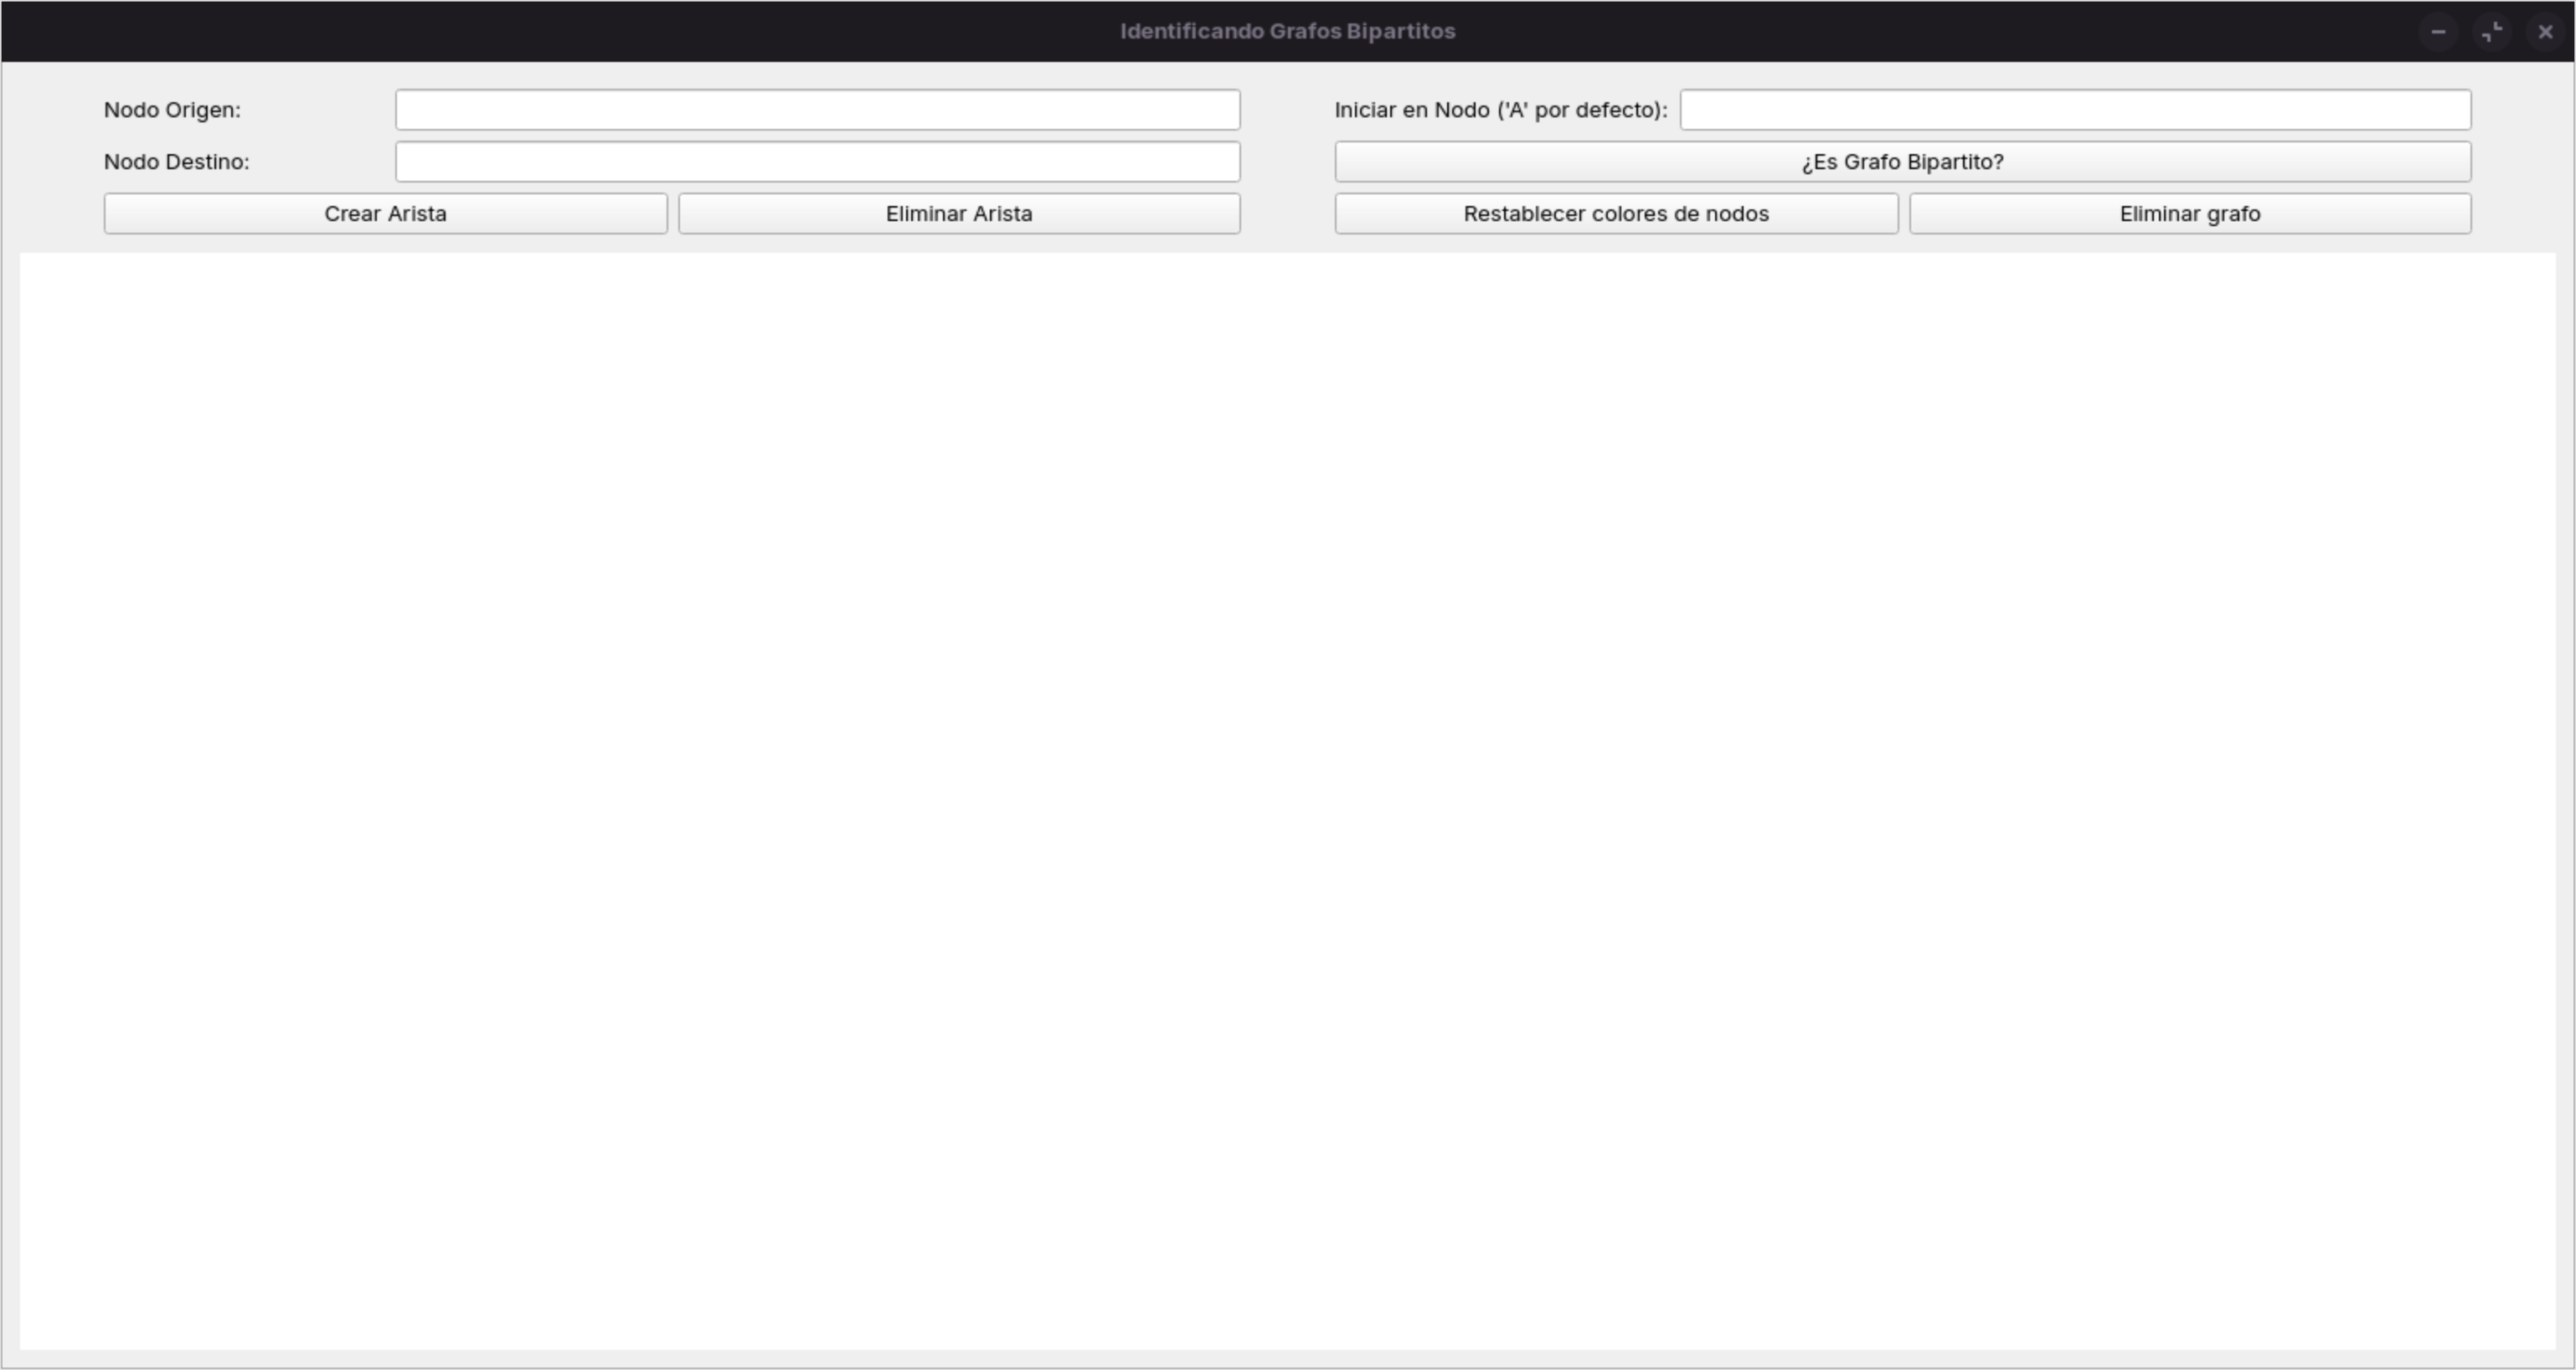
\includegraphics[width=0.5\textwidth]{images/menu.png} 
    \caption{Menú principal}
    \label{fig:menu}
\end{figure}

En la figura \ref{fig:creacion_grafo} se representa un ejemplo de cómo se agregan los nodos en el grafo, de manera sencilla como si de un pincel se tratara: con el puntero haciendo solamente click en algún lugar del recuadro blanco (tablero) hará que se agreguen nodos al grafo y se representará en el lugar en el que se hizo dicha acción.

\begin{figure}[htbp]
    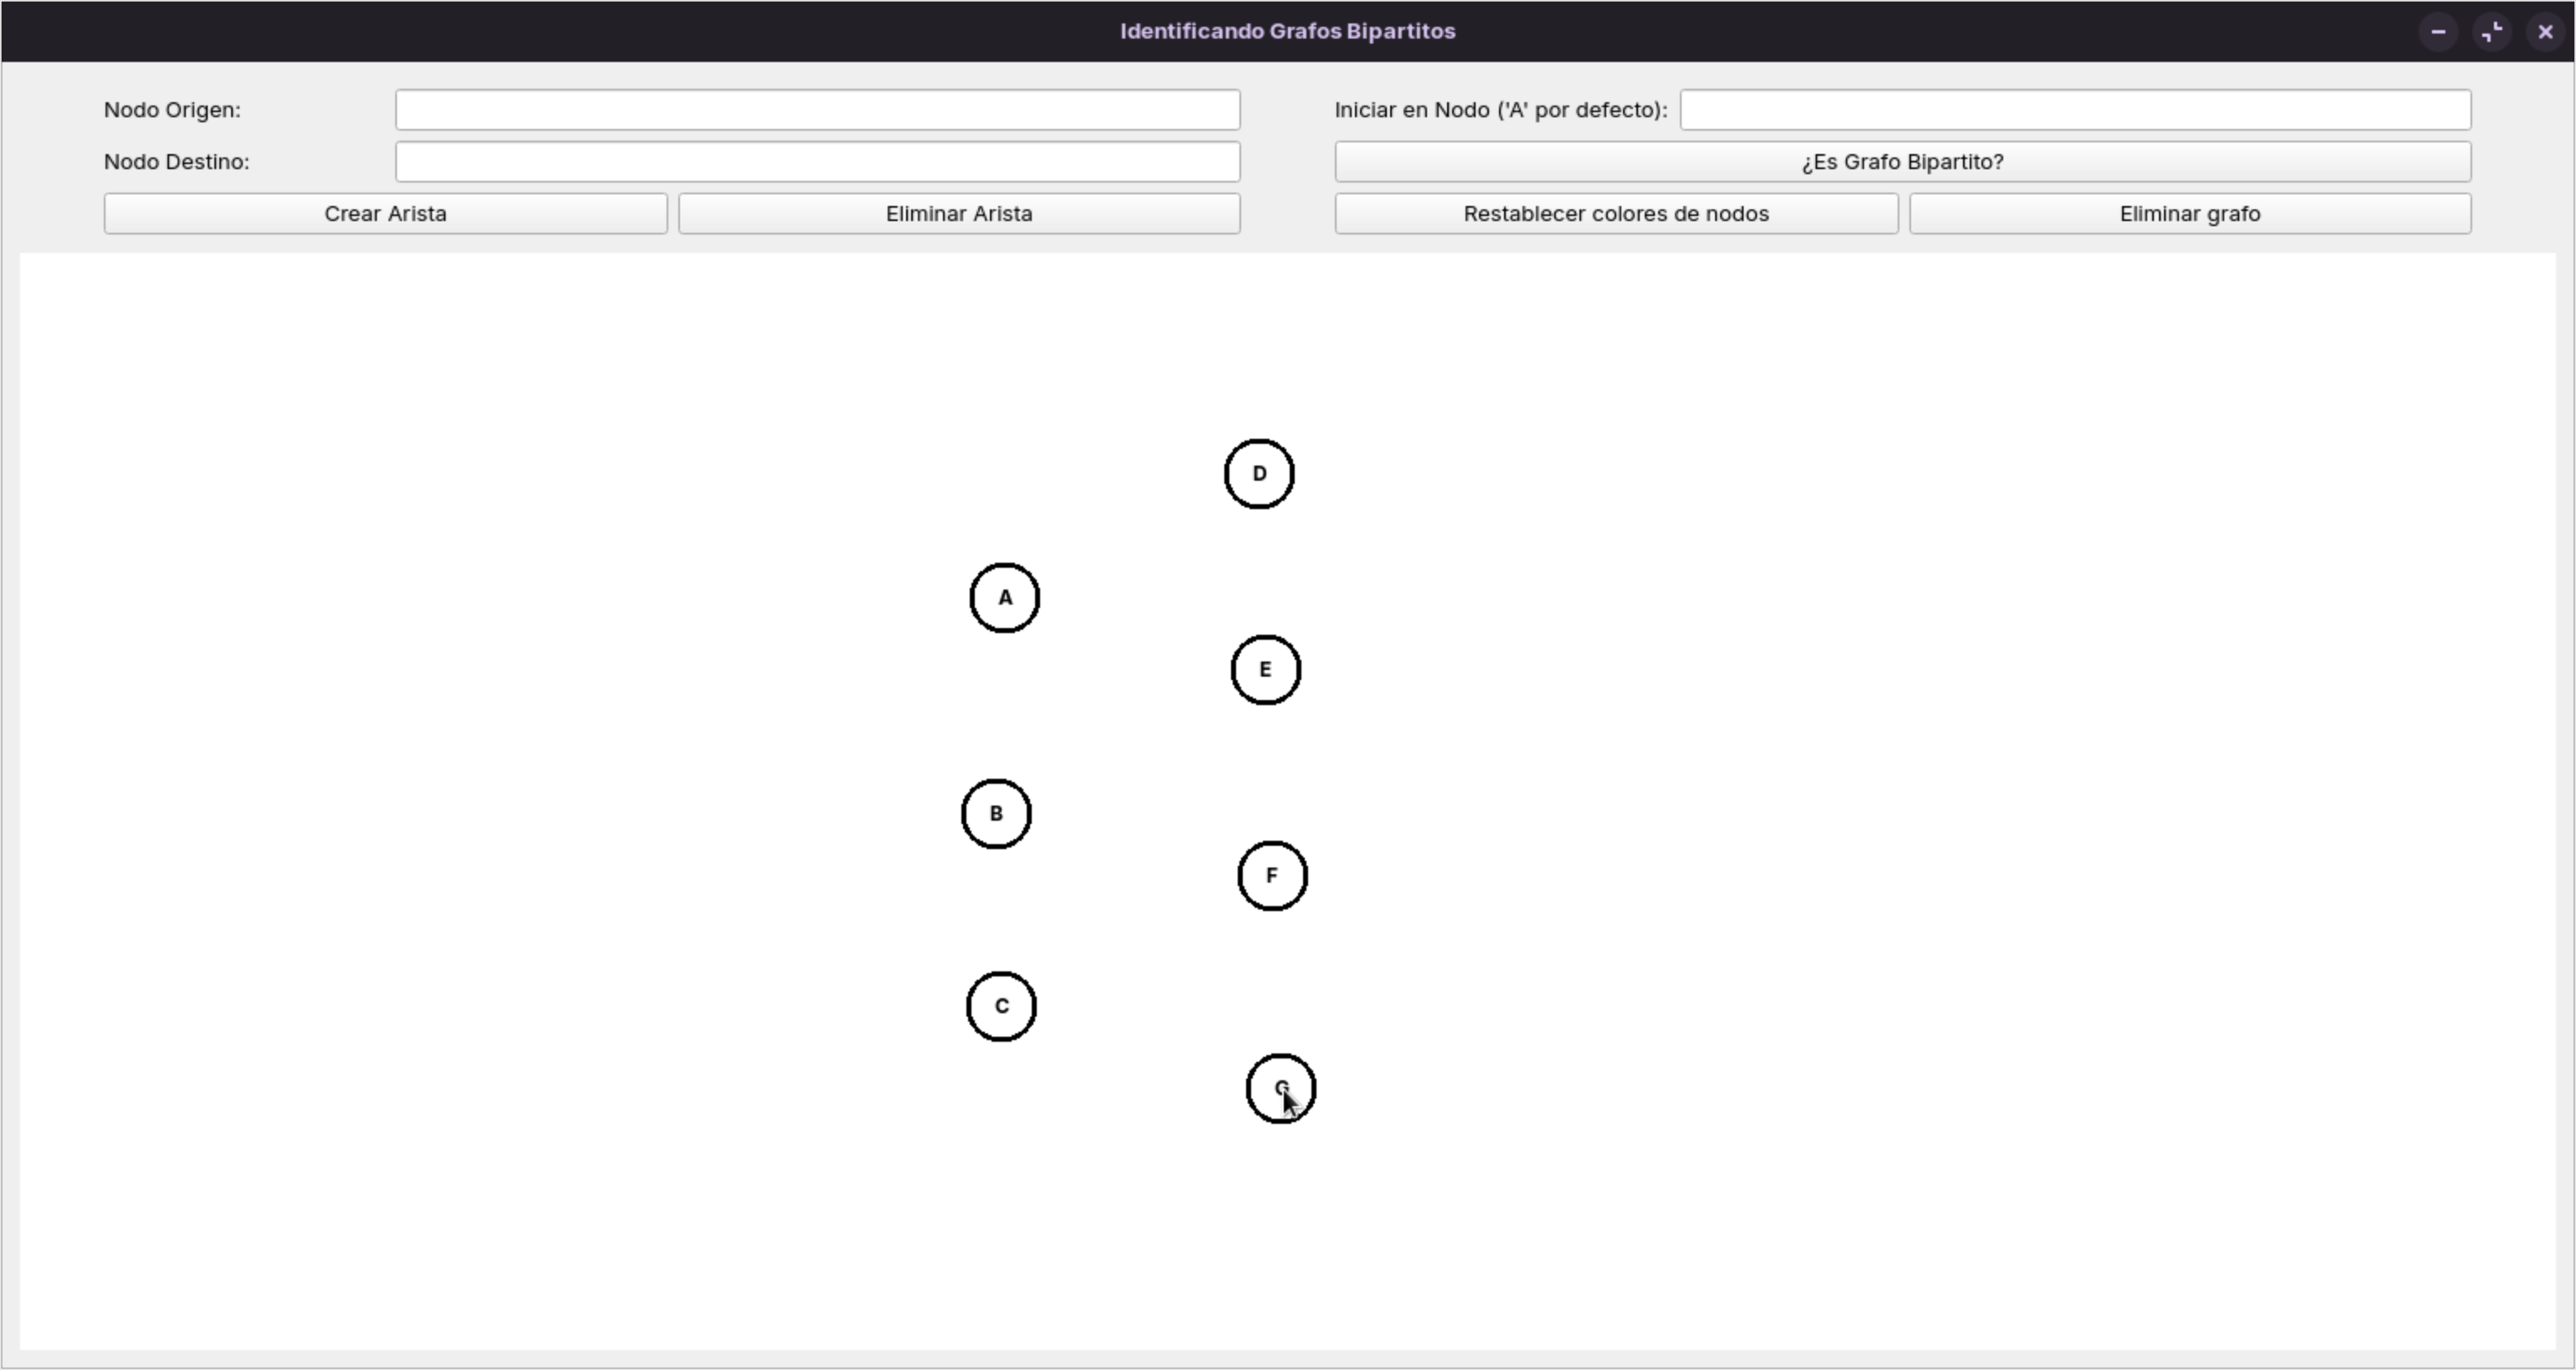
\includegraphics[width=0.5\textwidth]{images/creacion_grafo.png} 
    \caption{Creación de Grafo}
    \label{fig:creacion_grafo}
\end{figure}

Como se explicó anteriormente, los nodos tienen aristas de manera en que están tanto en el nodo A como en el nodo B, en la figura \ref{fig:creacion_aristas} demuestra esta misma funcionalidad, de manera en que para saber en que punto origen se tiene un punto destino para la creación de una arista, se deberá ingresar el valor de dicho nodo.

\begin{figure}[htbp]
    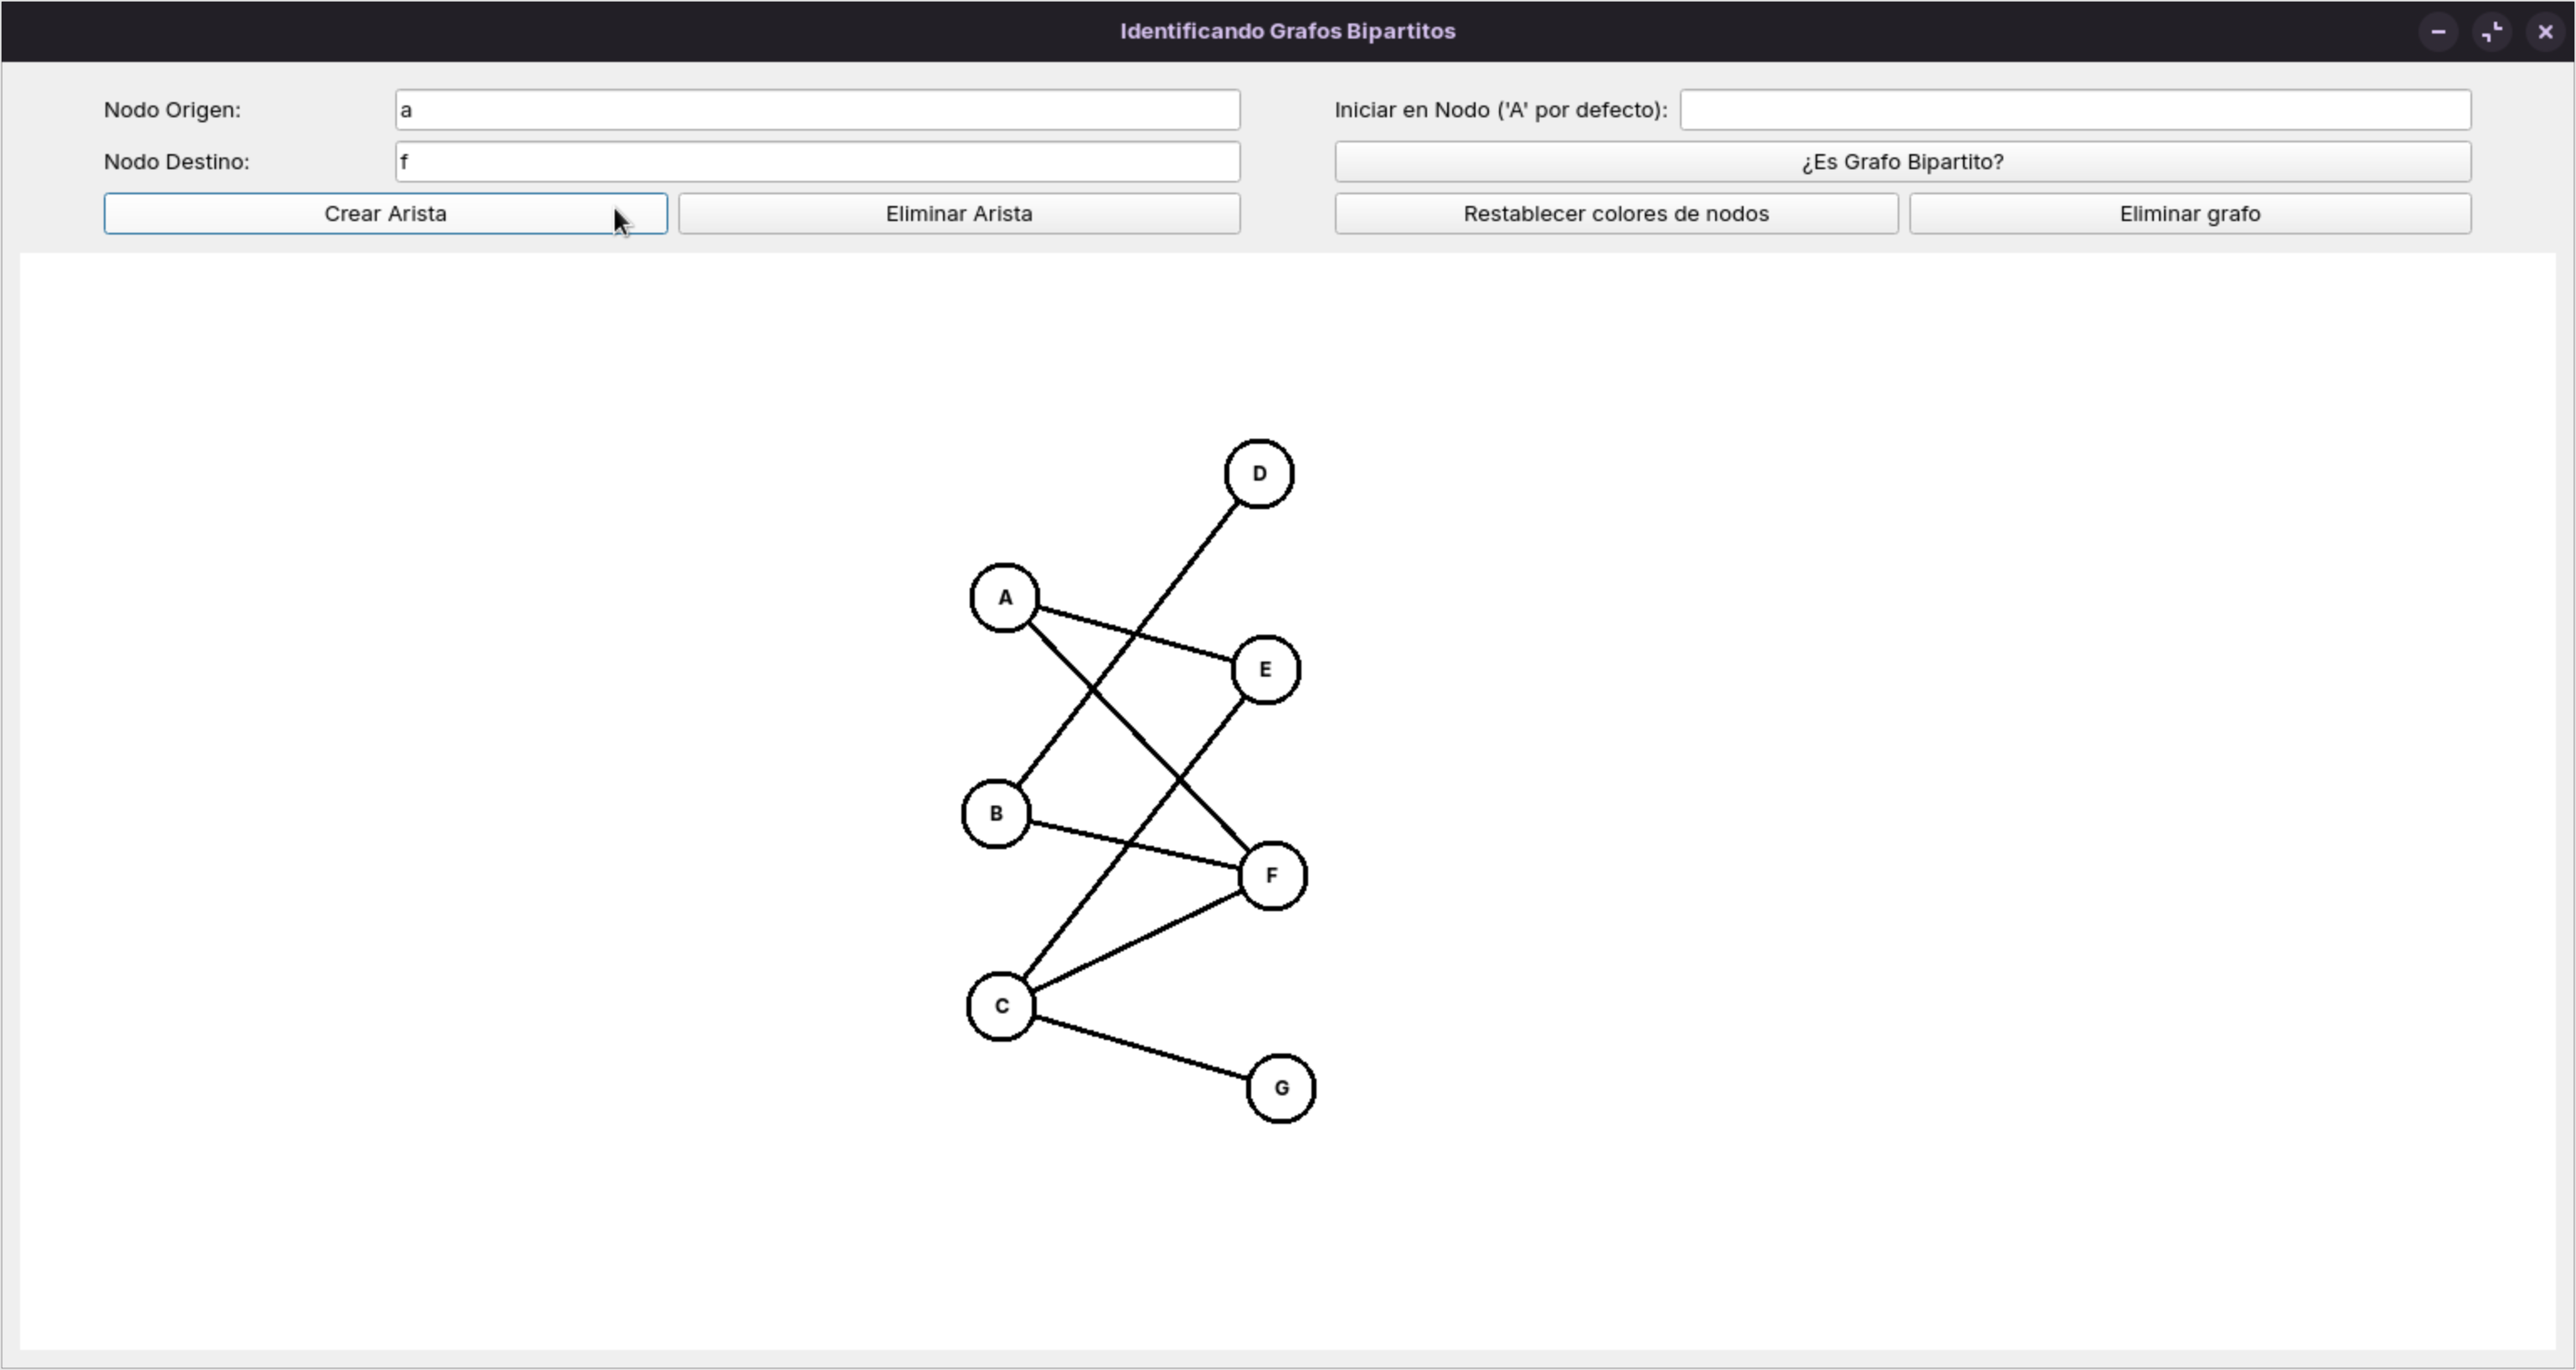
\includegraphics[width=0.5\textwidth]{images/creacion_arista.png} 
    \caption{Creación de Aristas}
    \label{fig:creacion_aristas}
\end{figure}

Con lo anterior realizado, ahora sí podemos ejecutar nuestro algoritmo de Grafo Bipartito presionando el botón ''¿Es Grafo Bipartito?'' de manera en que tiene como parámetro opcional recibir desde que nodo se quiere partir, en dado caso que no se ingrese algún valor del nodo inicio, entonces se realizará apartir del primer elemento que se haya agregado en primera instancia (es decir, el nodo 'A') de manera en que se guardará este primero en un conjunto 'A', al visitar sus vecinos estos estarán en guardados en un conjunto 'B' y serán marcados como ''visitados'' generando que no se imparta un error de bucle y sepamos identificar los nodos que han sido visitados, en la cual (dependiendo del grafo ingresado) mostrará por mensaje en una venta mencionando si el gafo es o no un Grafo Bipartito. La figura \ref{fig:grafo_bipartito} demuestra un ejemplo de la secuencia visual de esto mismo.

\begin{figure}
\subfloat[Iniciación en Nodo 'A']{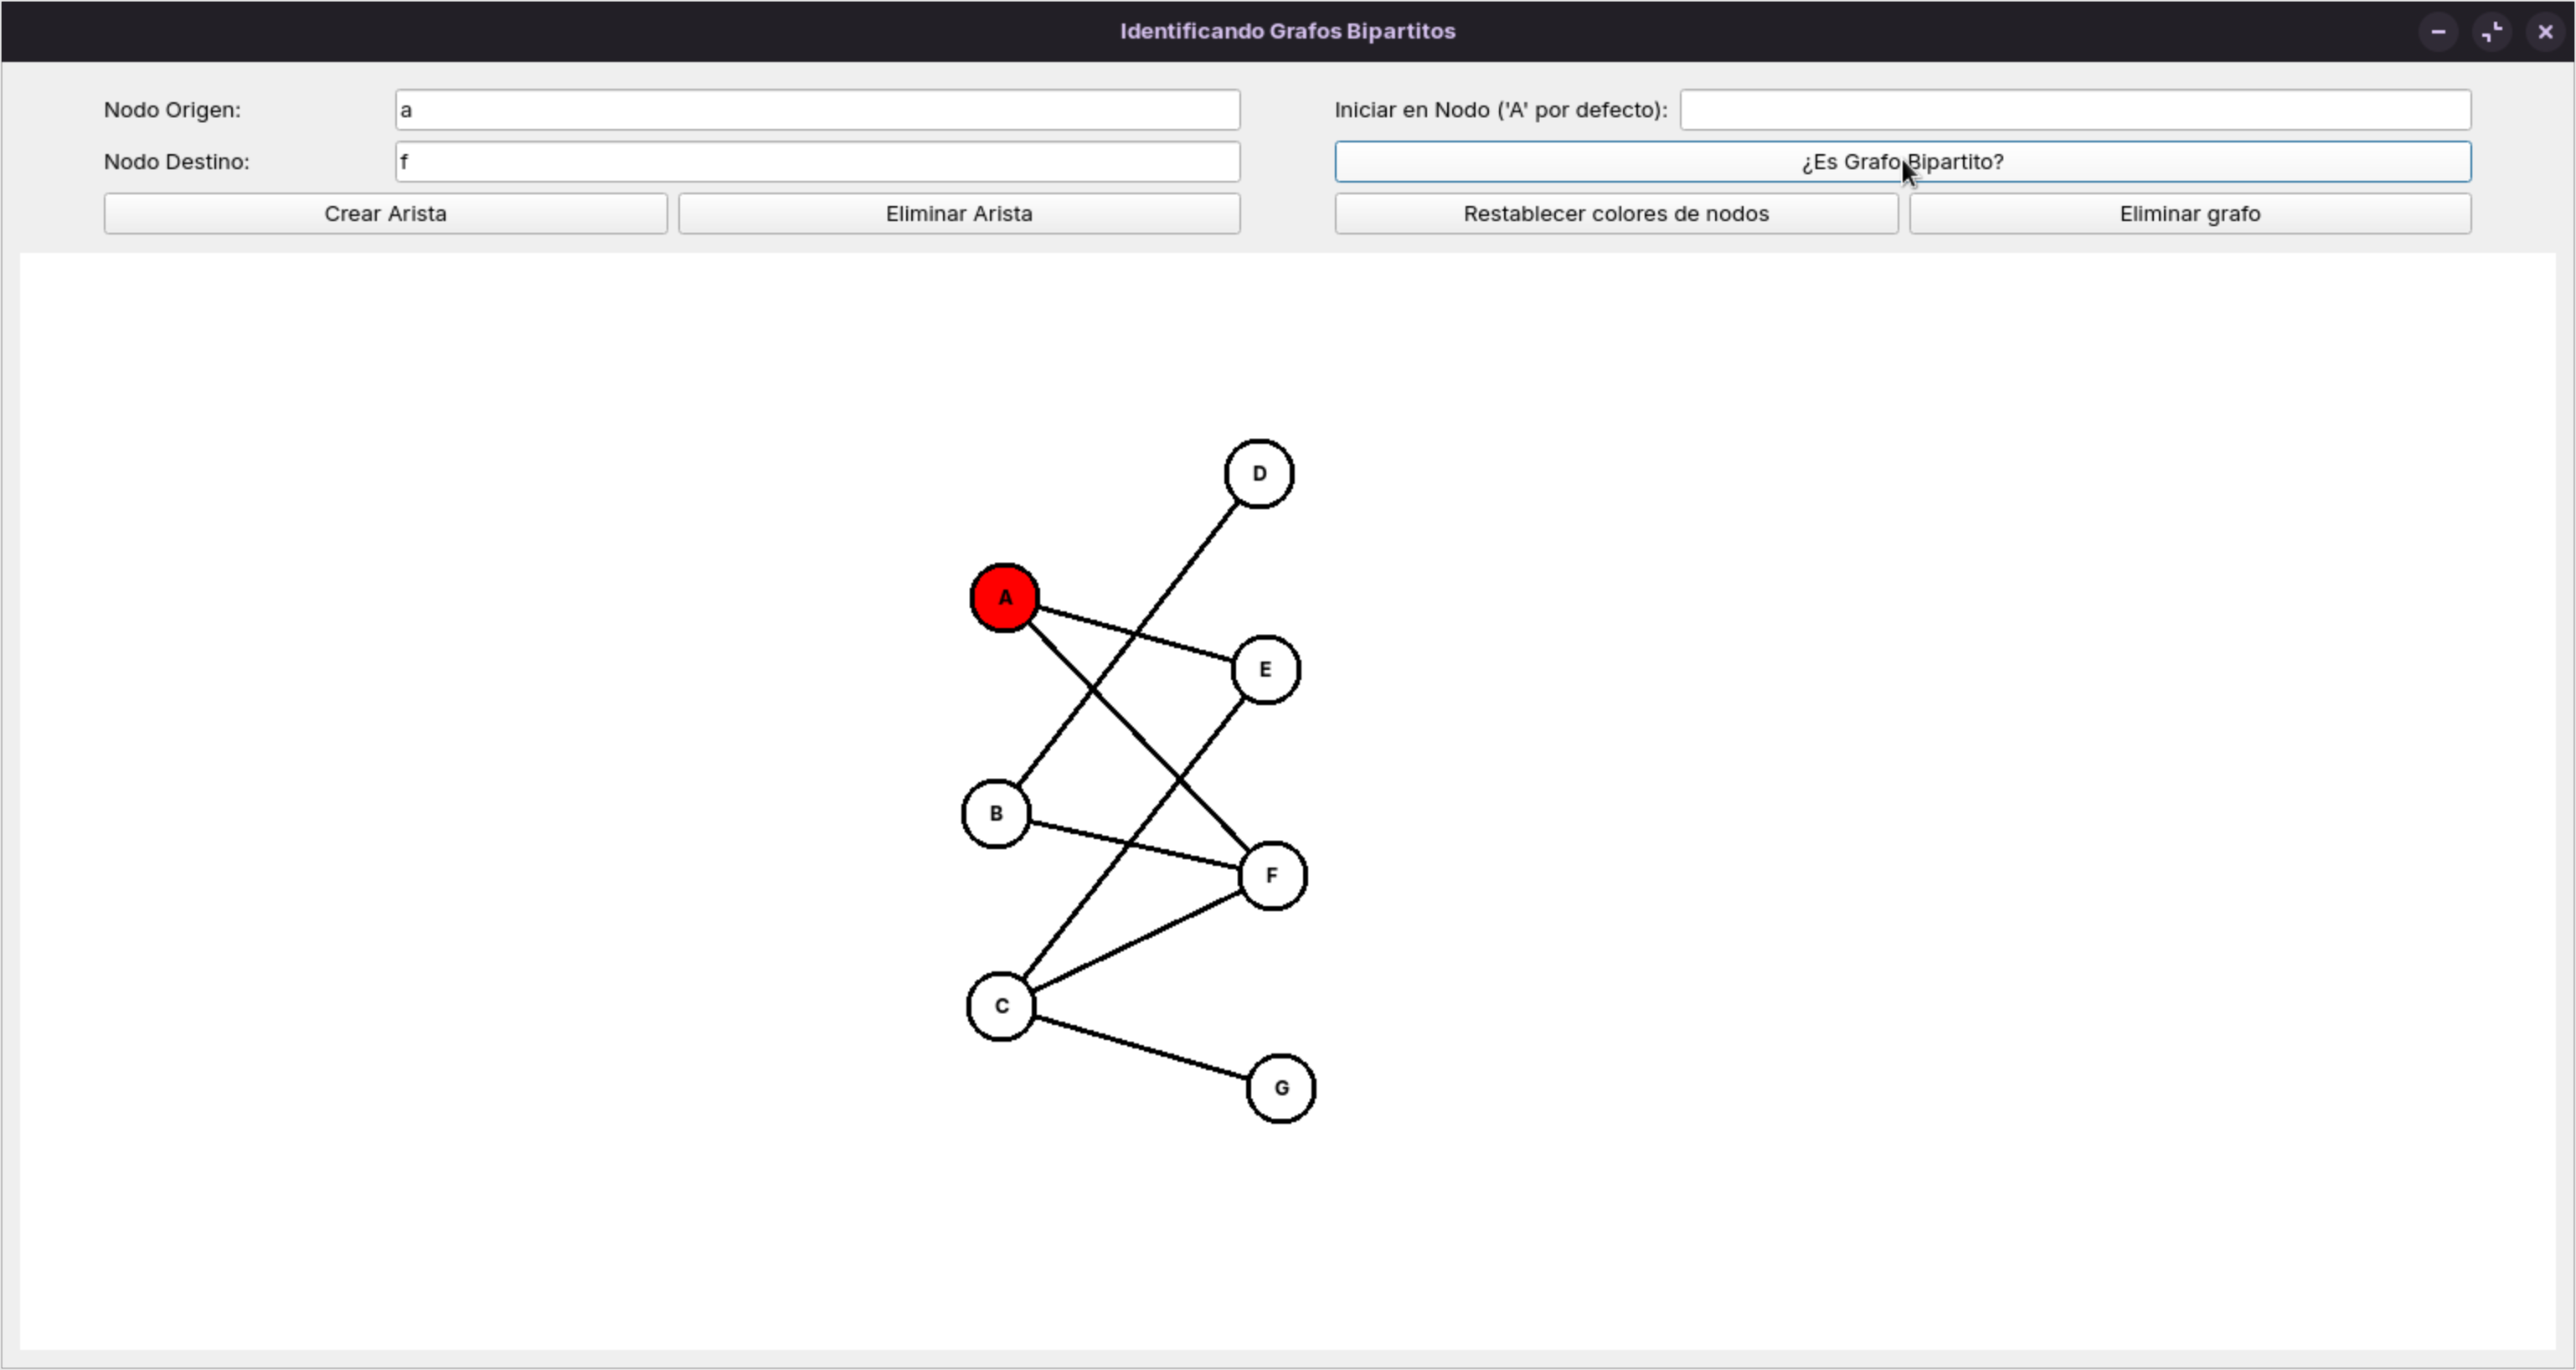
\includegraphics[width=\breite\columnwidth]{images/sec1.png}}\\
\subfloat[Visita en vecinos]{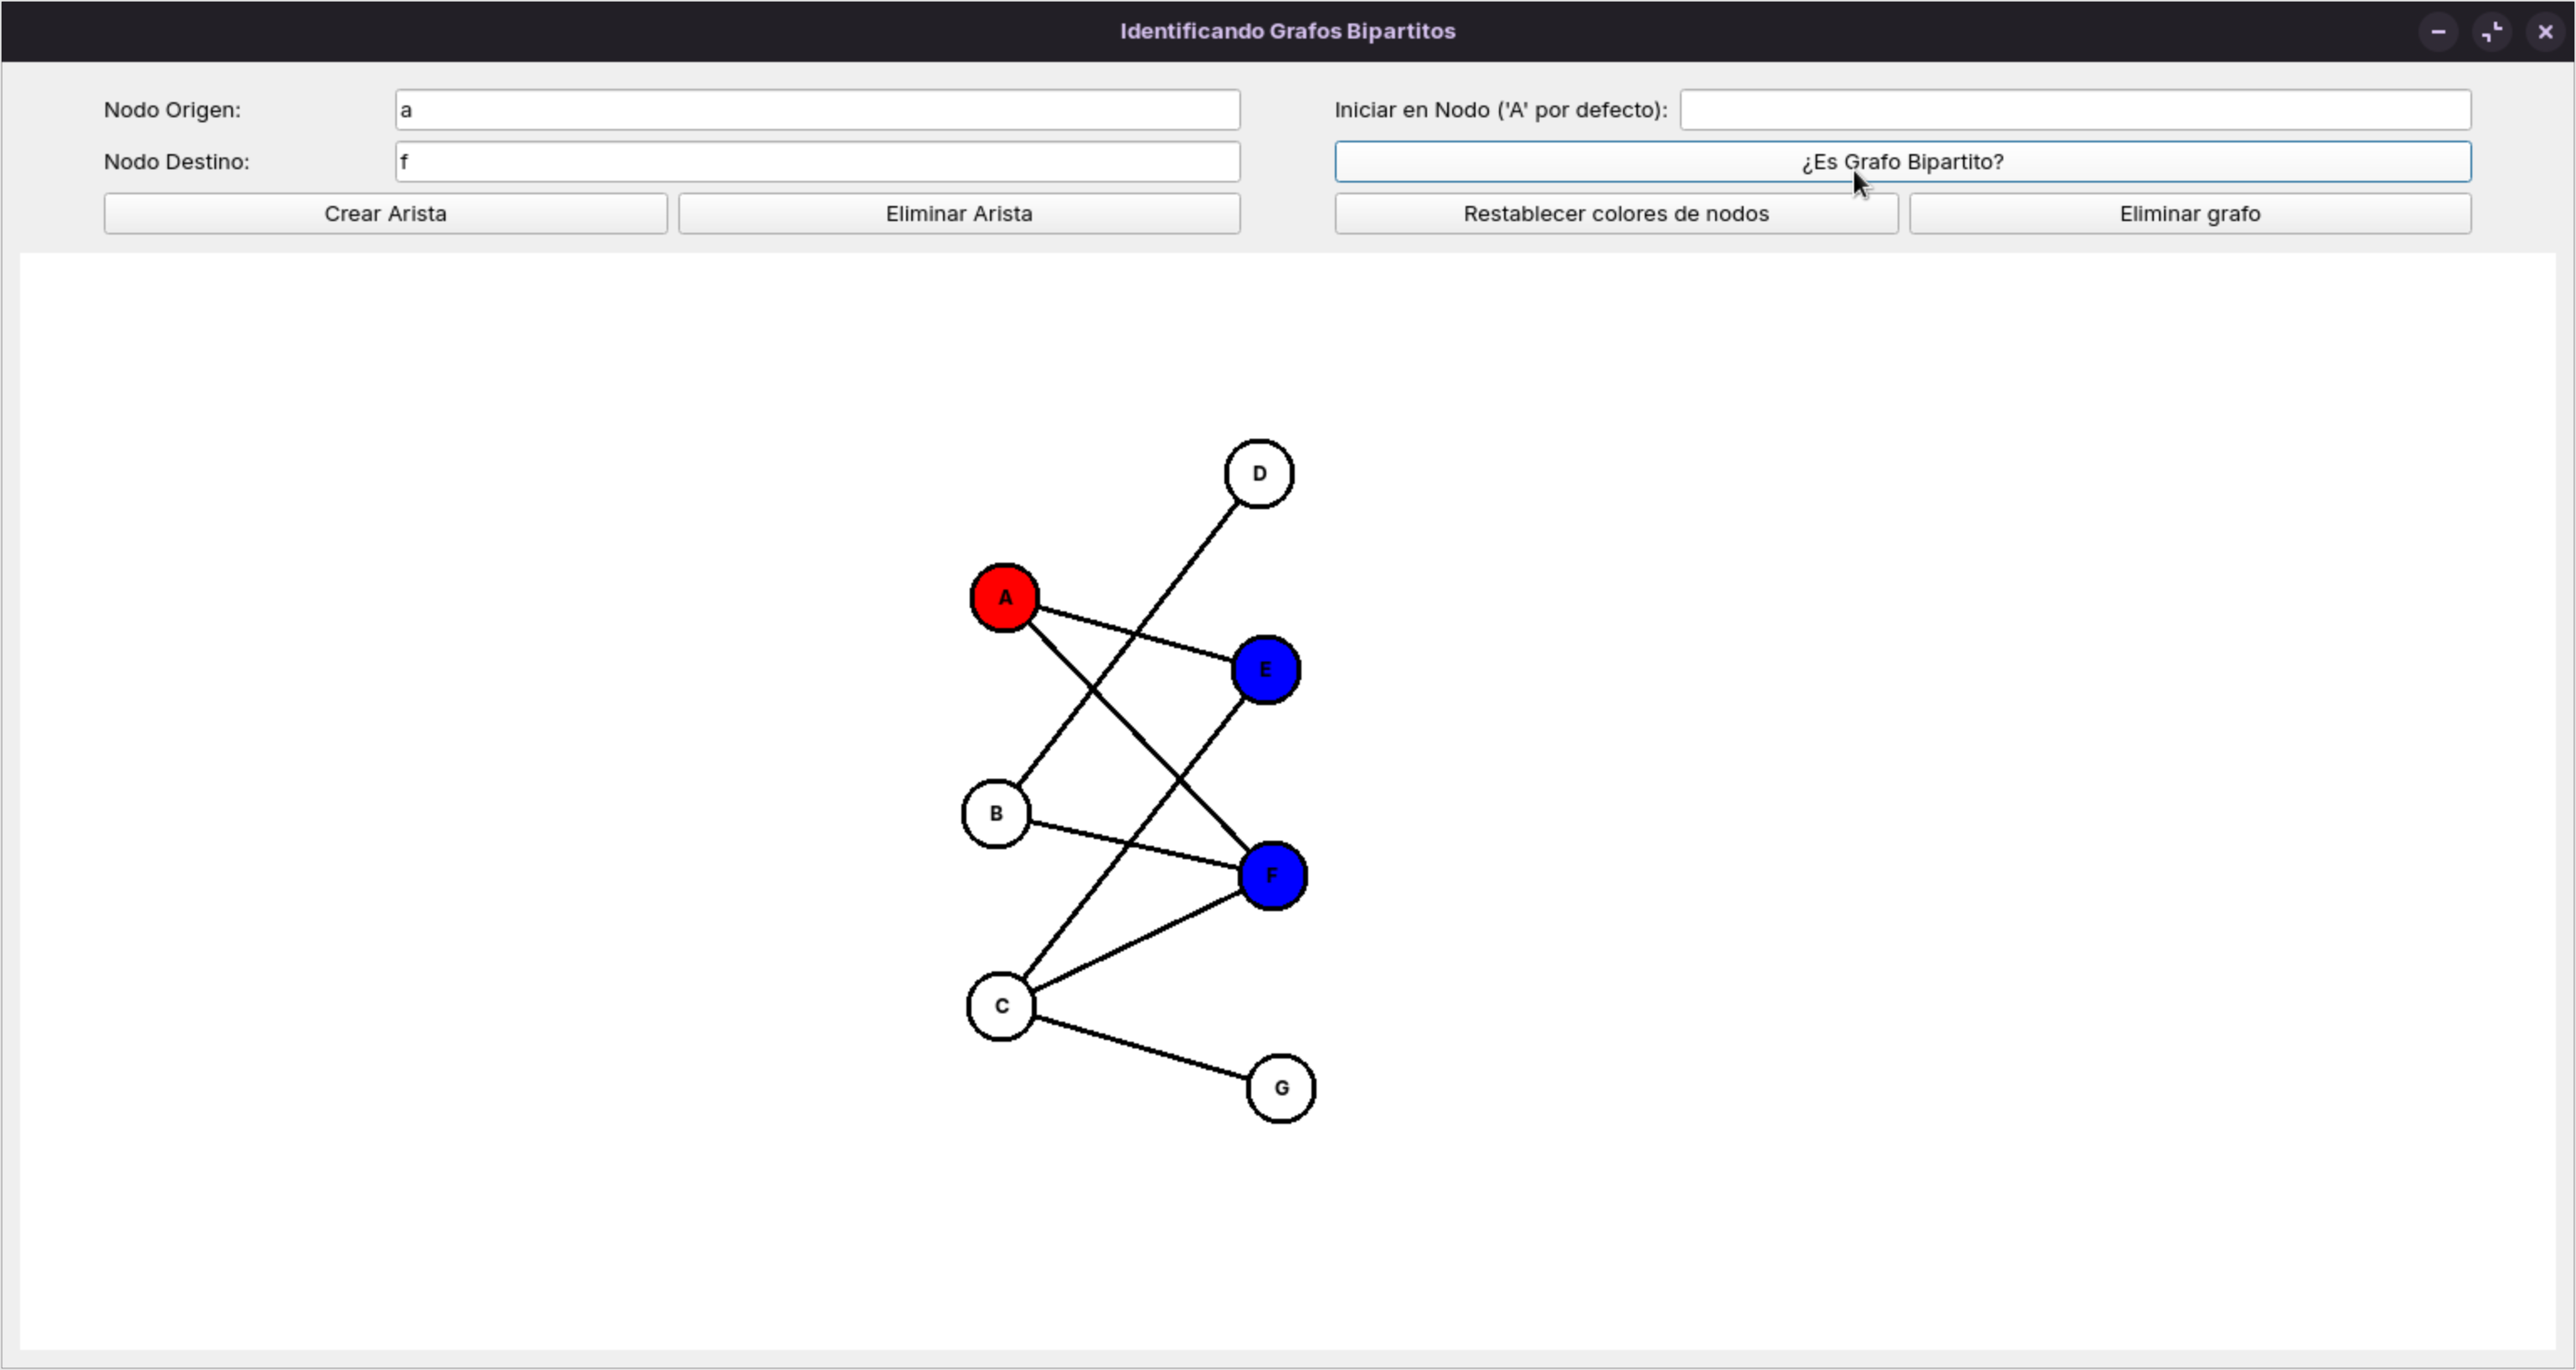
\includegraphics[width=\breite\columnwidth]{images/sec2.png}}\\
\subfloat[Resultados]{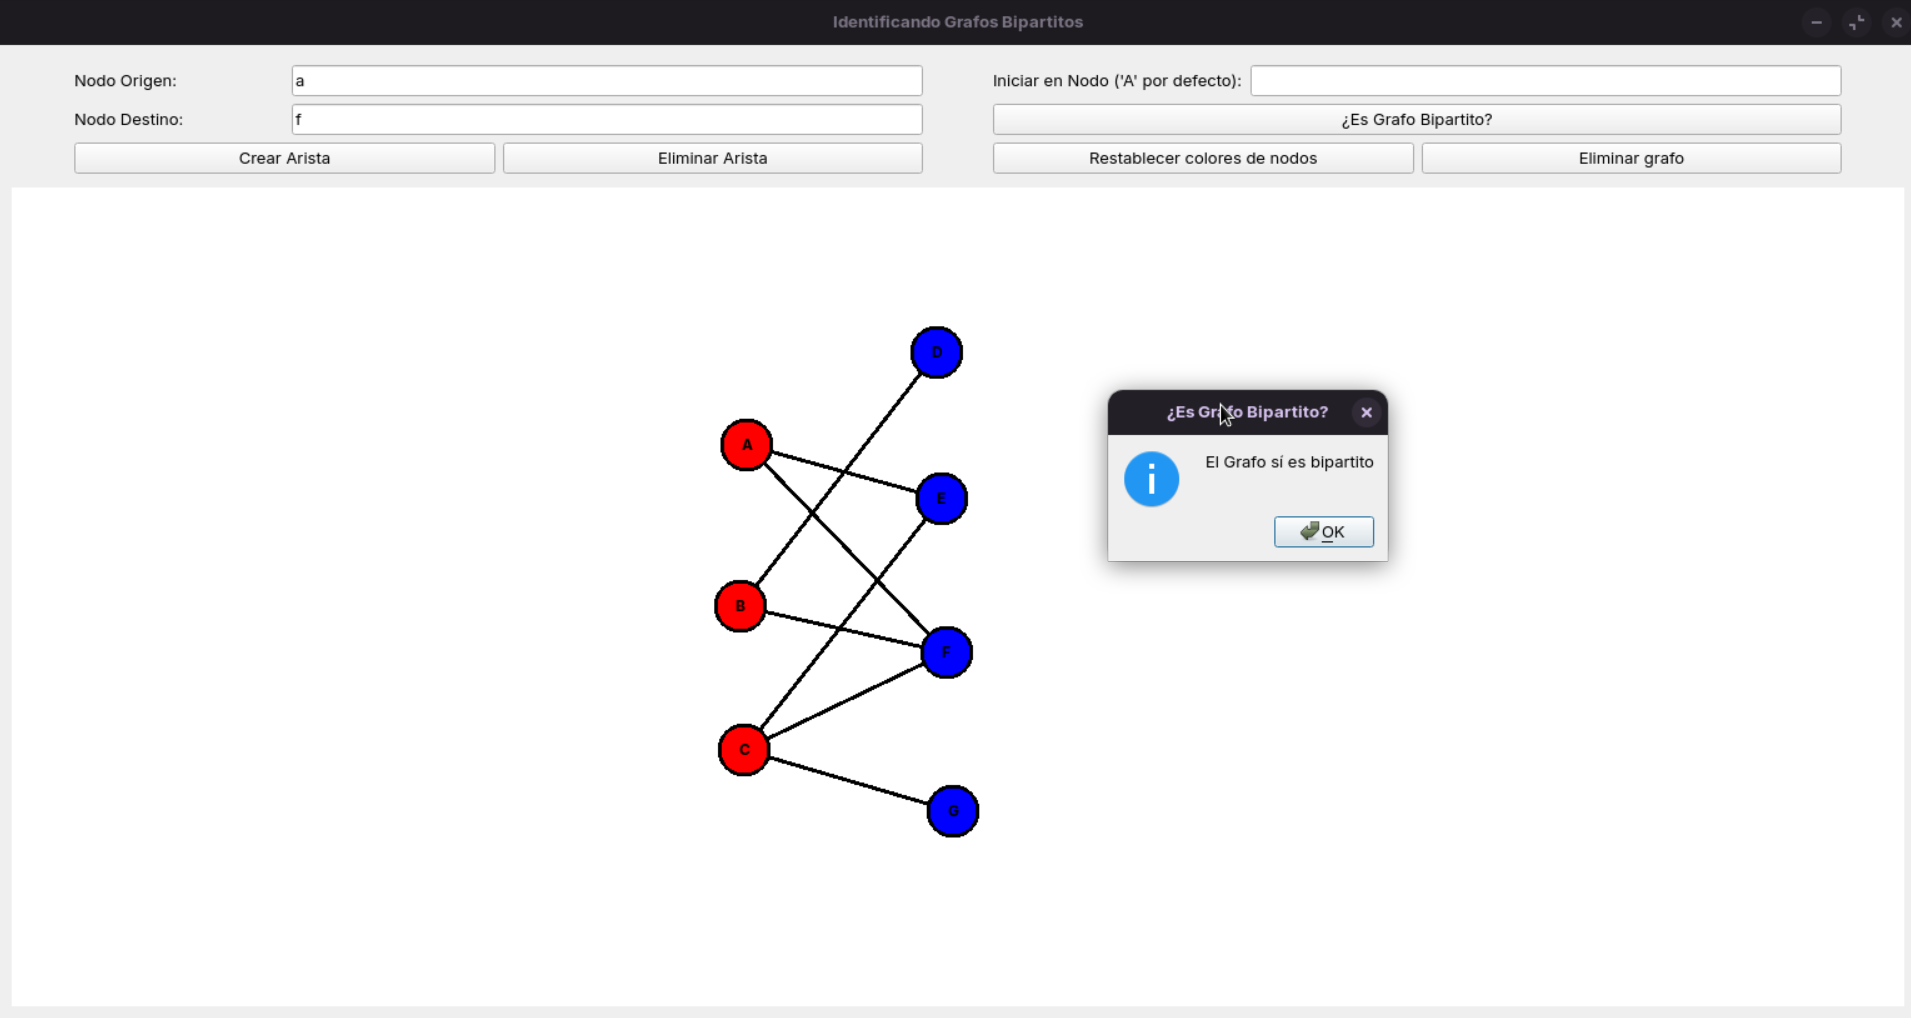
\includegraphics[width=\breite\columnwidth]{images/sec3.png}}\\
\caption{Grafo Bipartito}
\label{fig:grafo_bipartito}
\end{figure}

En el caso en el que el gafo ingresado no sea un grafo bipartito, entonces, se terminará la representación visual y se mostrará un mensaje en pantalla informando acerca de esto mismo, en la figura \ref{fig:no_bipartito} se demuestra un ejemplo.

\begin{figure}[htbp]
    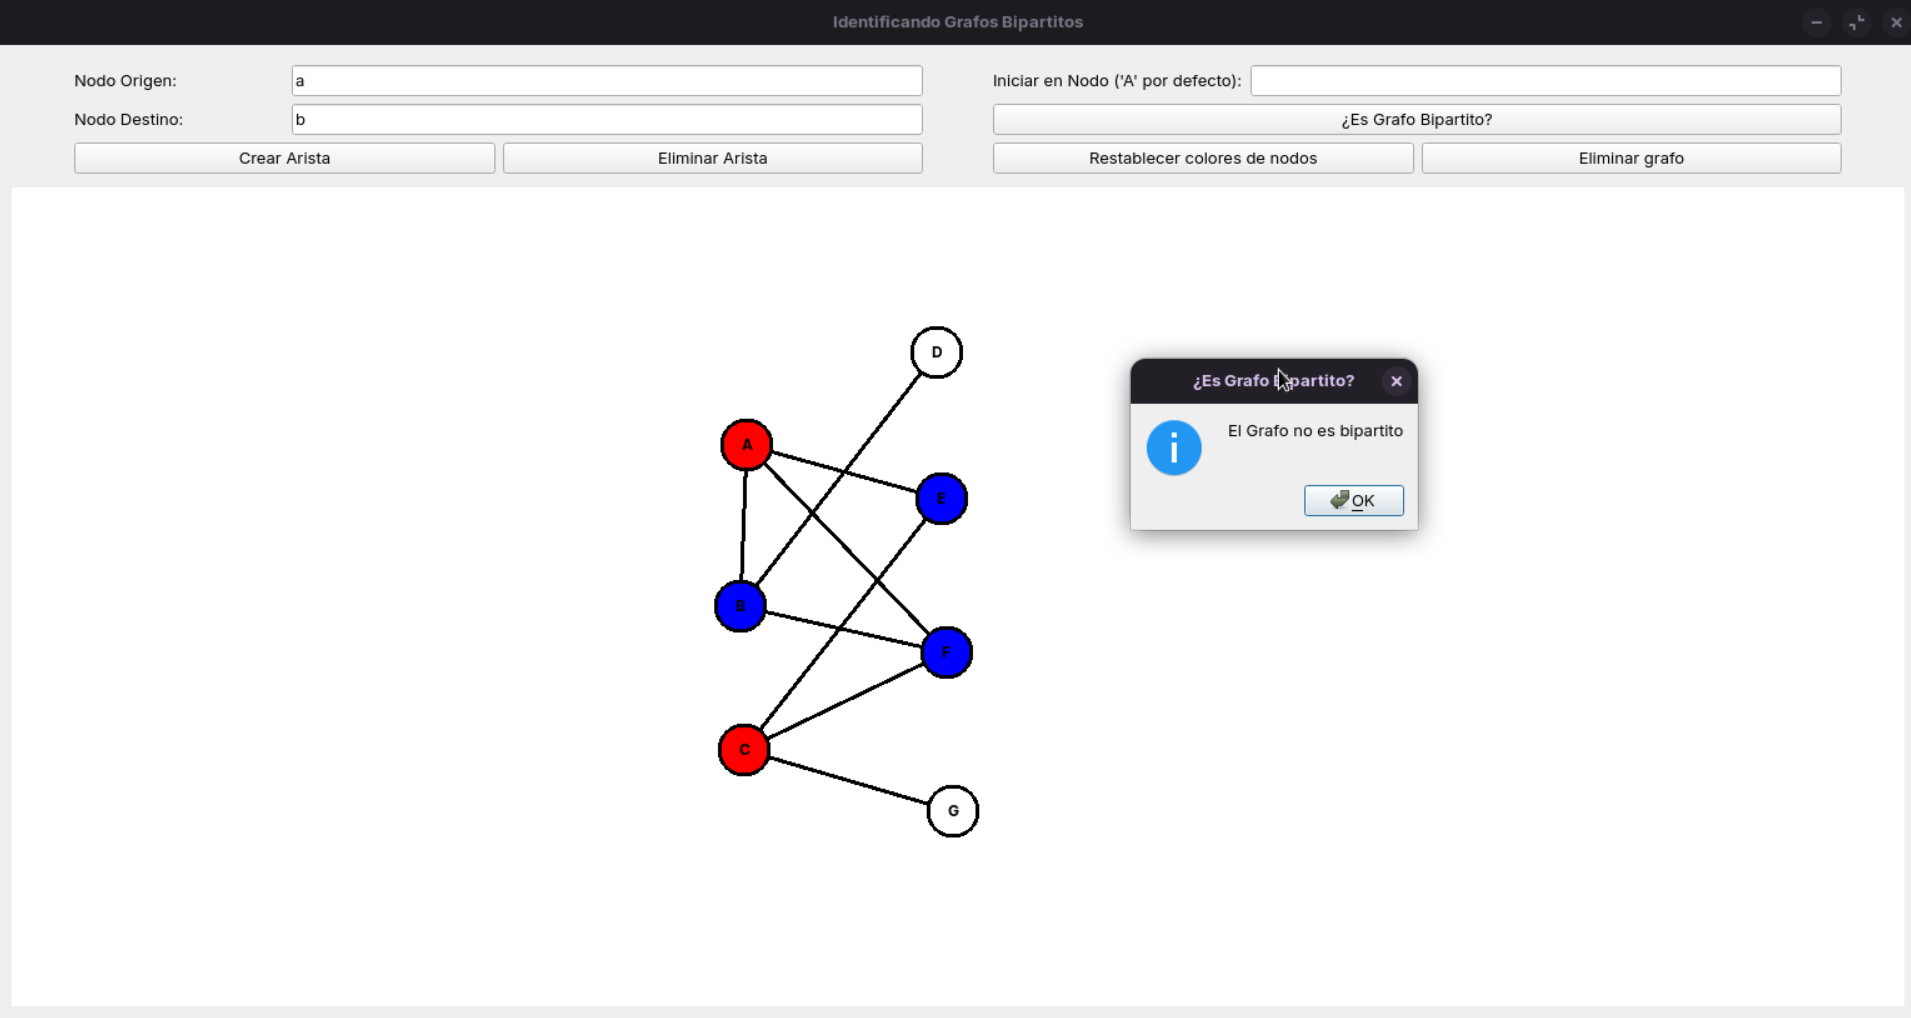
\includegraphics[width=0.5\textwidth]{images/no_bipartito.png} 
    \caption{Grafo No Bipartito}
    \label{fig:no_bipartito}
\end{figure}

El resto de funcionalidades sirven de aprovechamiento para evitar tener que regenerar un grafo en caso de que haya ocurrido un error en la conexión de un nodo a otro, facilitando así la experiencia del uso impartido de este proyecto, en la figura \ref{fig:otras_opciones} se demuestran los casos de usos de estos mismos.

\begin{figure}
\subfloat[Restablecimiento de colores de los nodos]{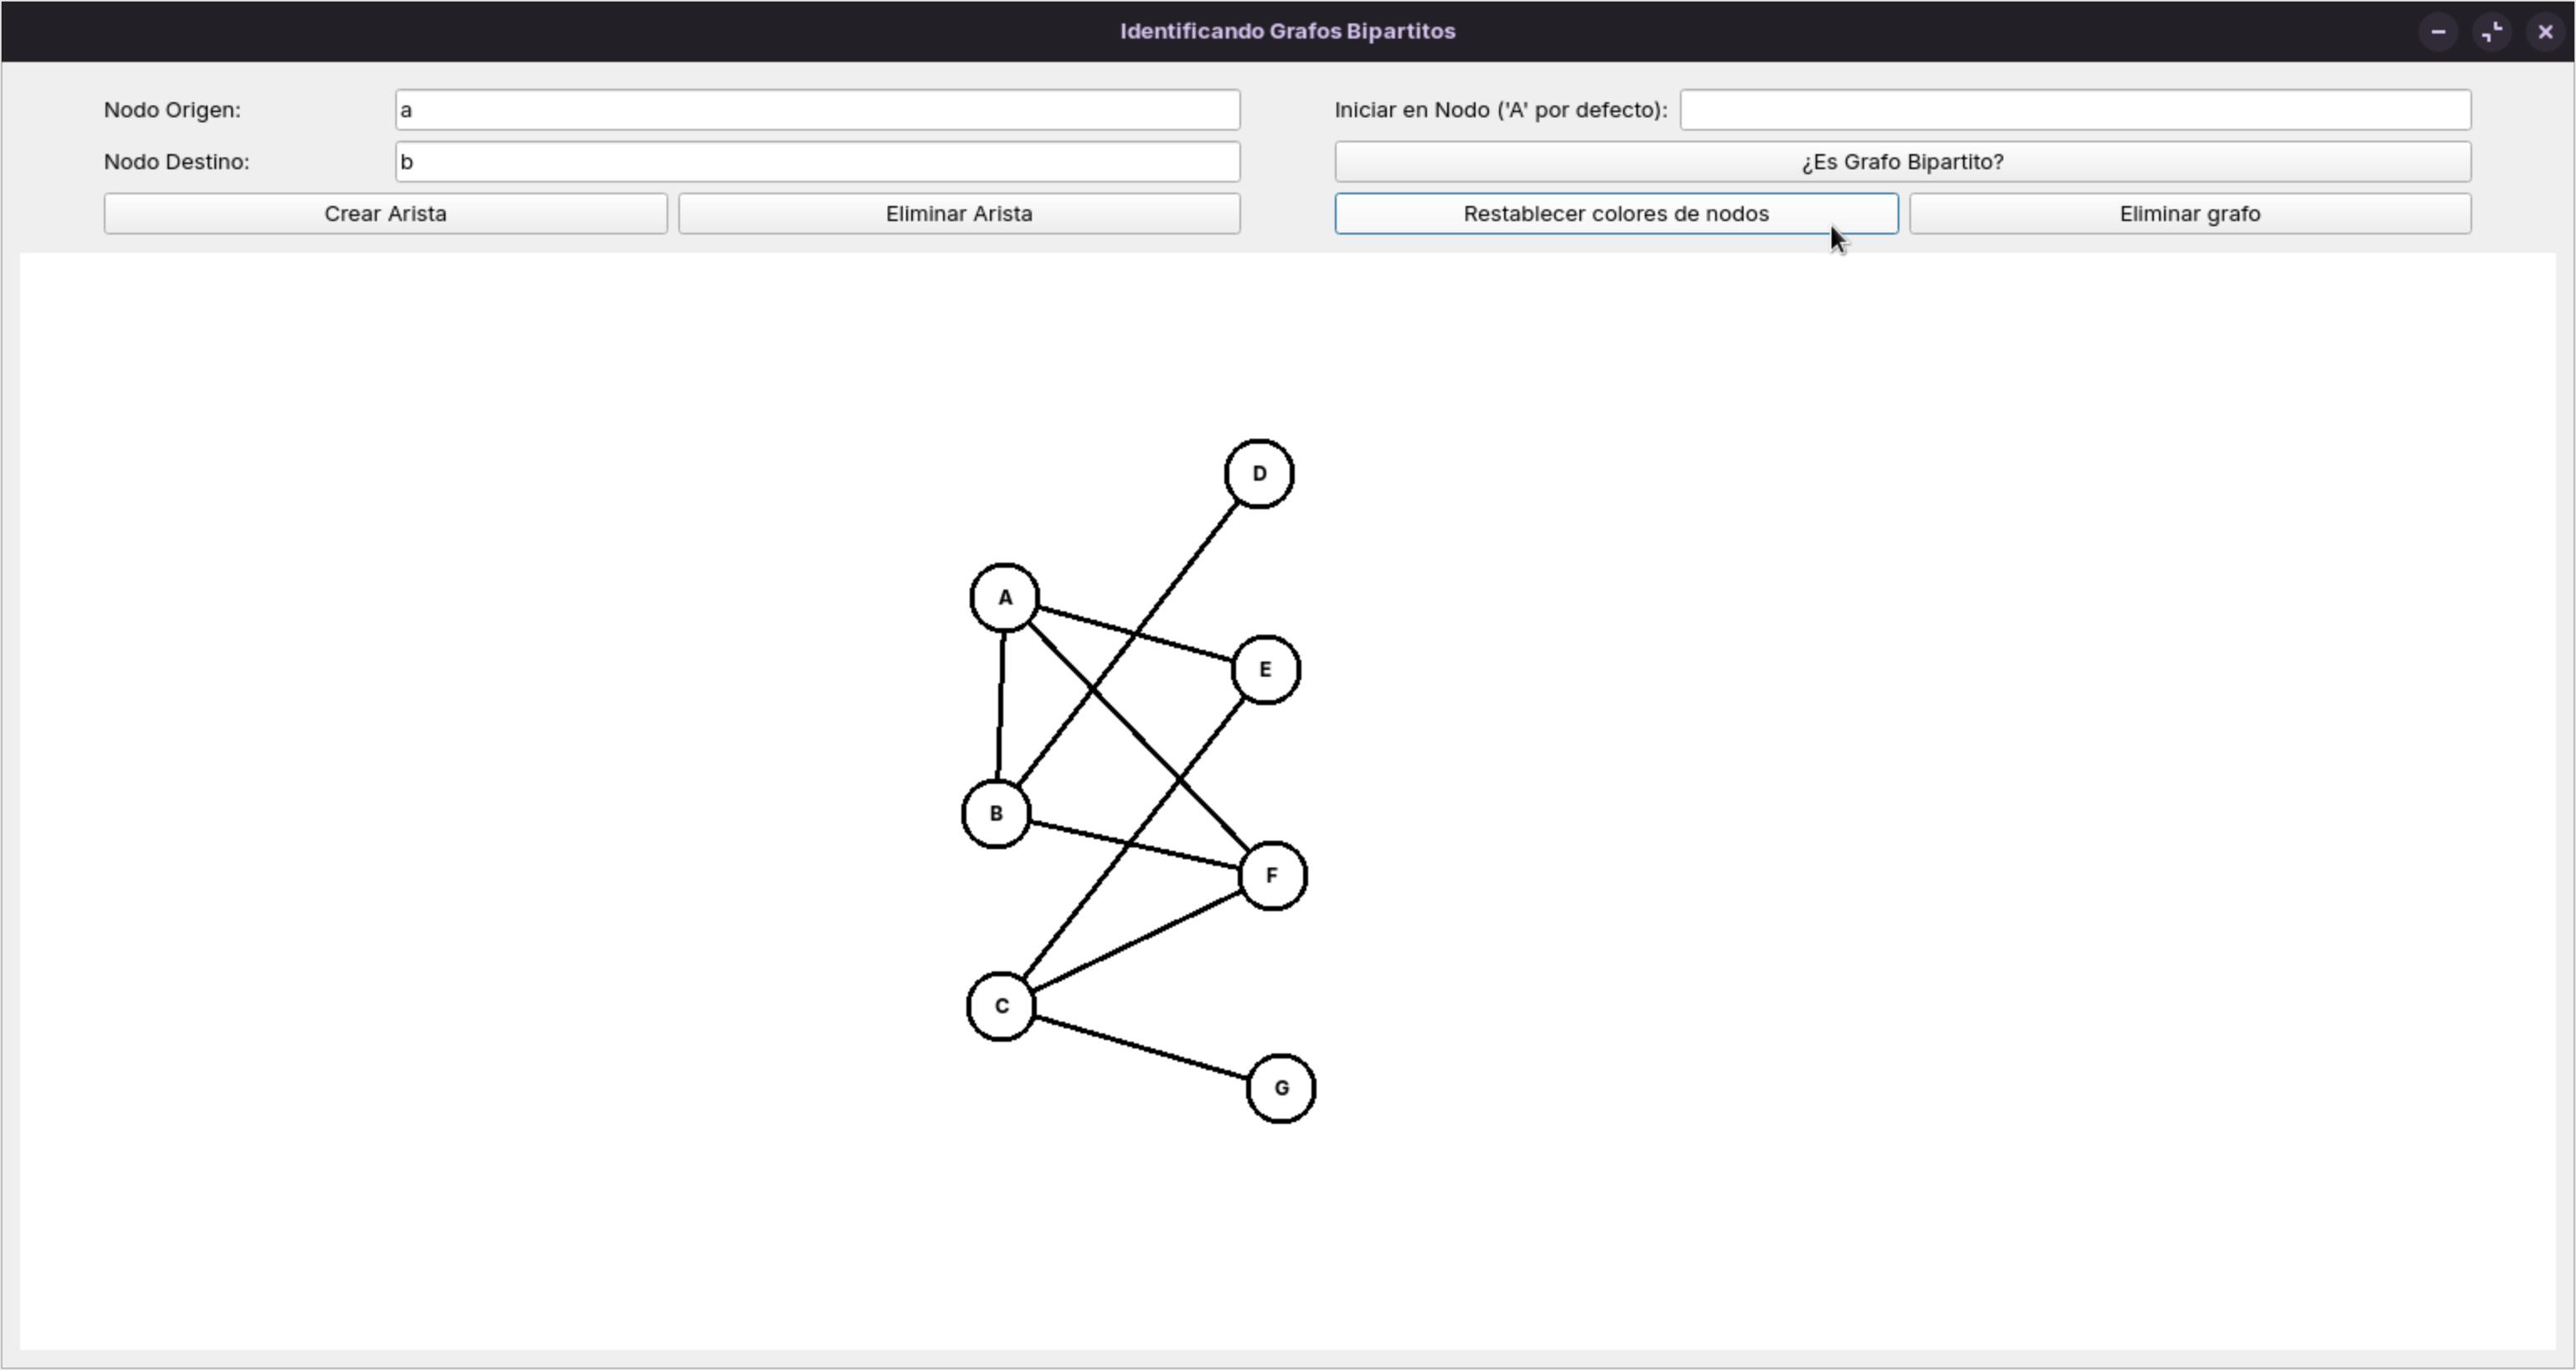
\includegraphics[width=\breite\columnwidth]{images/restablecer_colores.png}}\\
\subfloat[Eliminación de arista]{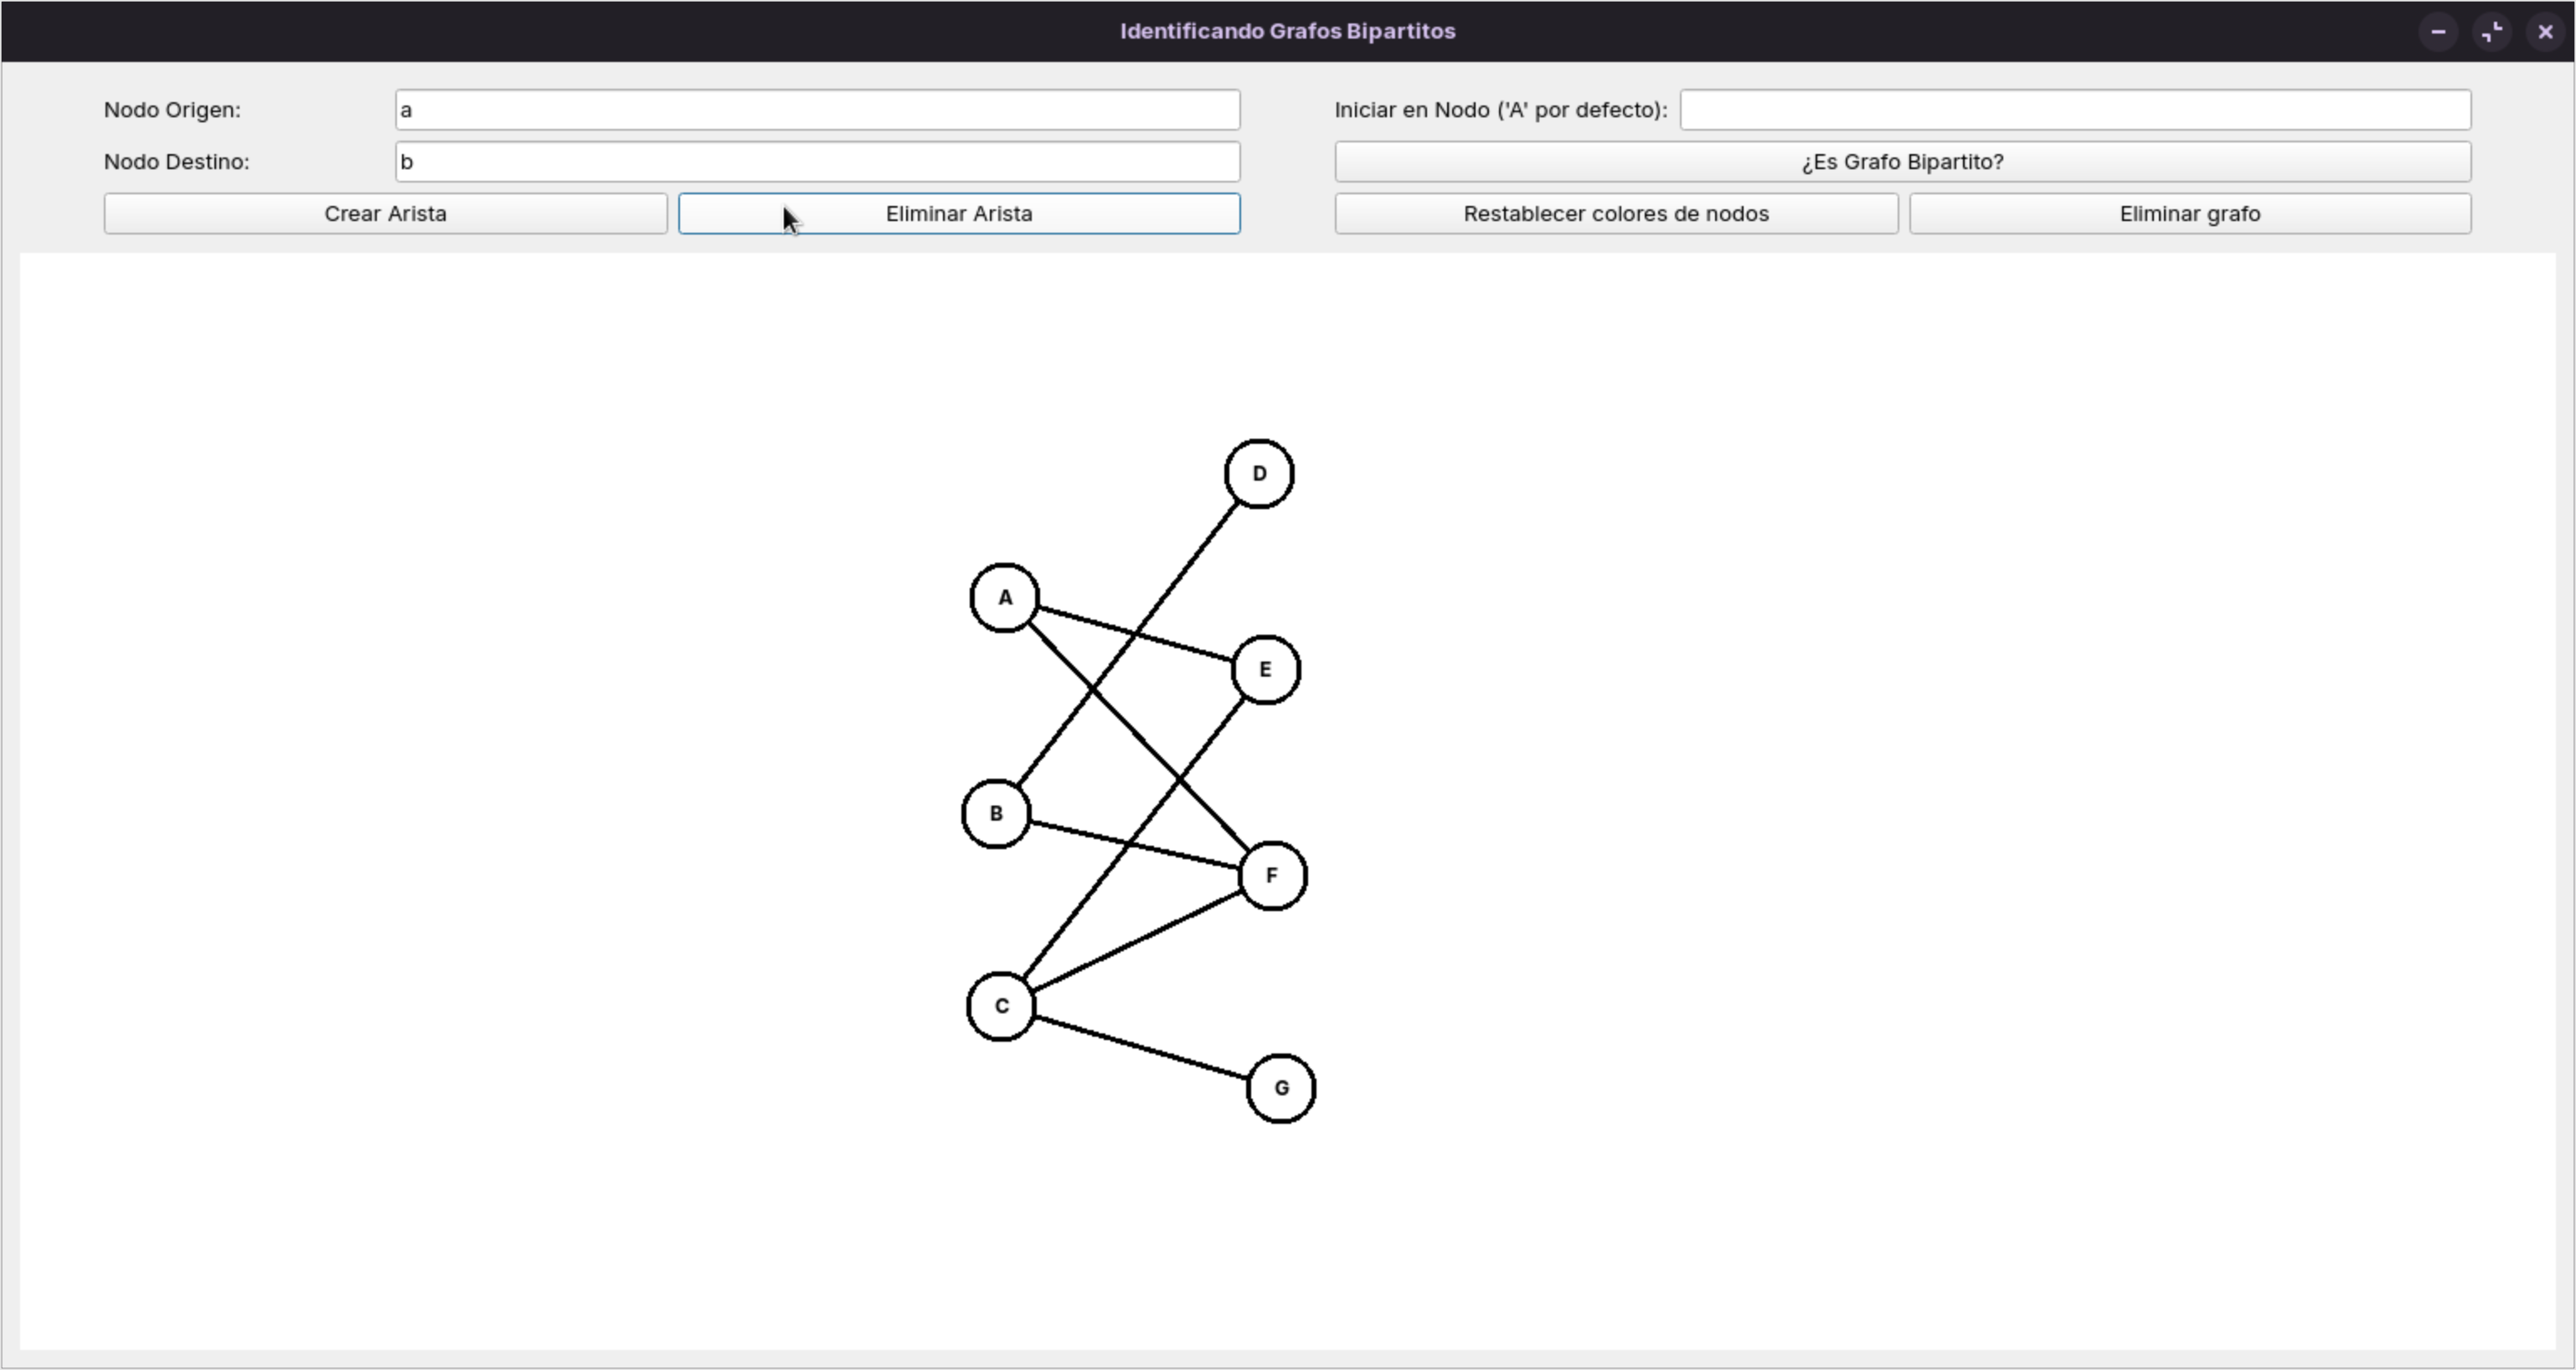
\includegraphics[width=\breite\columnwidth]{images/eliminar_arista.png}}\\
\subfloat[Eliminación de grafo]{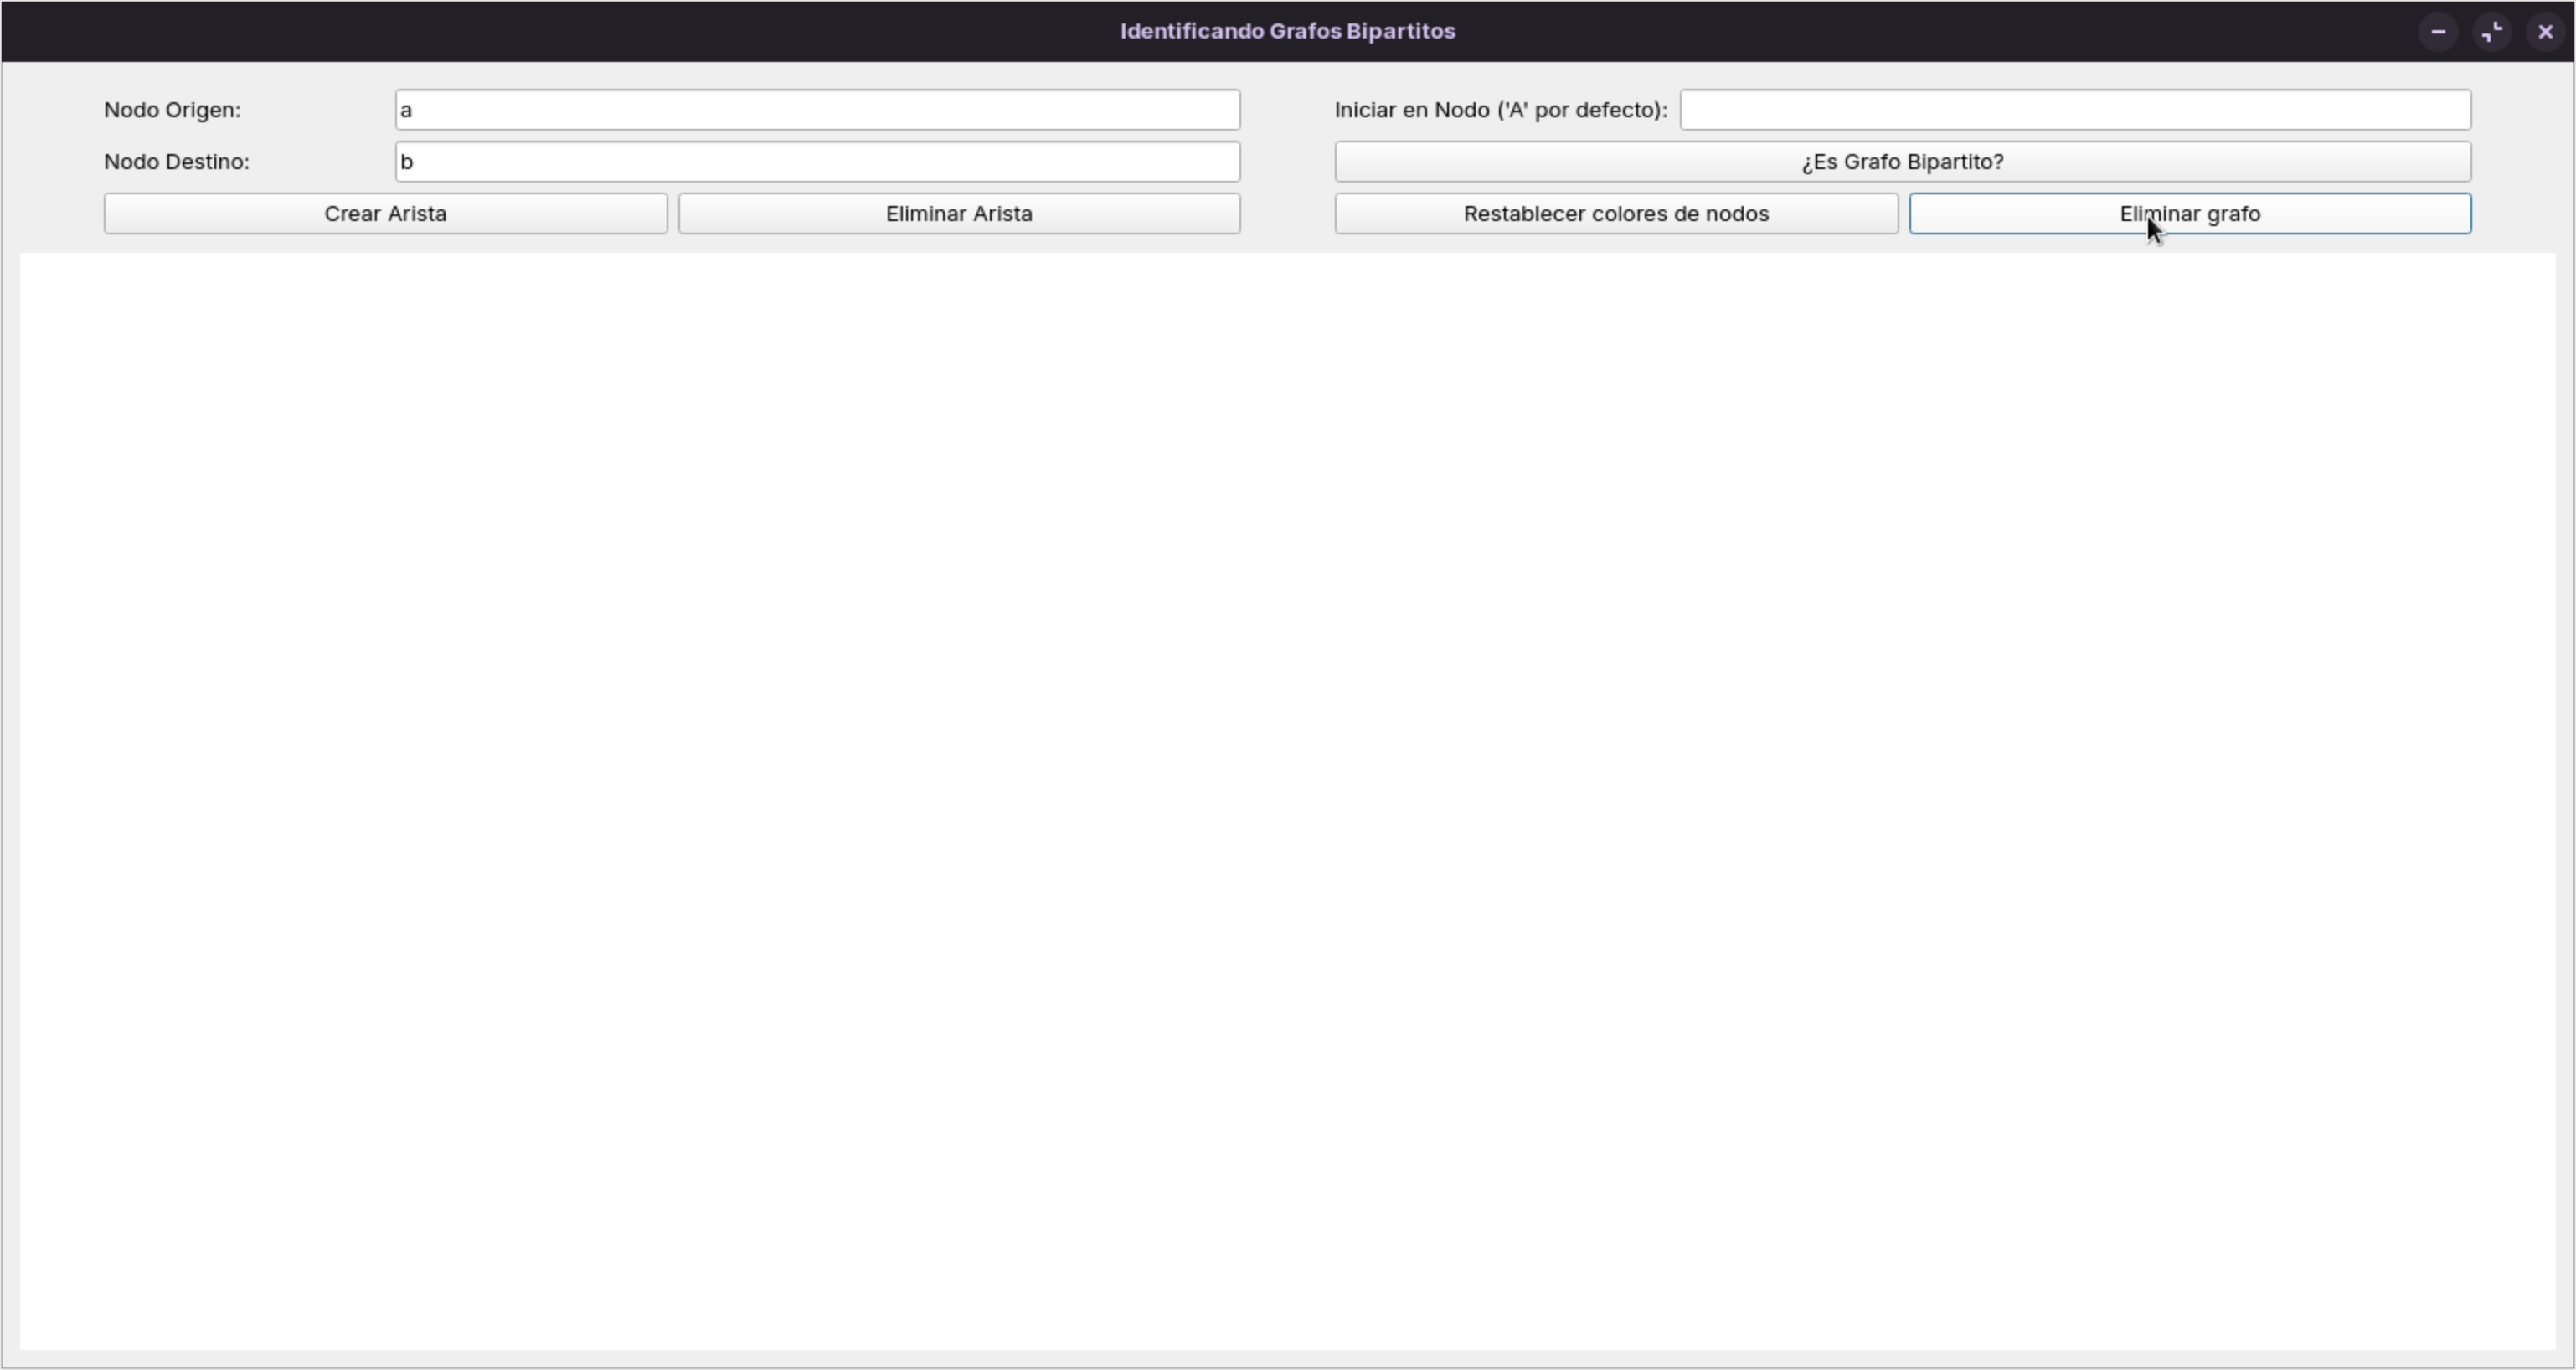
\includegraphics[width=\breite\columnwidth]{images/eliminar_grafo.png}}\\
\caption{Grafo Bipartito}
\label{fig:otras_opciones}
\end{figure}

\section{Conclusión}
La conclusión de este proyecto destaca la importancia de comprender y visualizar el algoritmo de Grafos Bipartitos. Los grafos en general son una estructura de datos fundamental en ciencias de la computación y matemáticas, utilizados para modelar una variedad de problemas del mundo real, desde redes sociales hasta rutas de transporte, así como en ciertas áreas de la programación o incluso de redes de computadoras.

Específicamente, los Grafos Bipartitos tienen aplicaciones en áreas como la teoría de grafos, la optimización, la planificación de horarios, la asignación de recursos y más. Su propiedad de poder dividir los nodos en dos conjuntos independientes los hace especialmente útiles en problemas donde se necesita asignar recursos de manera eficiente sin conflictos.

La visualización del algoritmo de Grafos Bipartitos no solo facilita la comprensión del algoritmo en sí mismo, sino que también proporciona una herramienta útil para educación y análisis de problemas que involucran grafos bipartitos. Además, este proyecto demuestra la capacidad de implementar algoritmos complejos de manera efectiva y presentarlos de una manera accesible y comprensible.

Para finalizar, este proyecto proporcionó conocimiento de manera exitosa al alumno, además de proporcionar resultados satisfactorios para la visualización de la ejecución de este algoritmo.

\addcontentsline{toc}{section}{Referencias} 
\printbibliography
%\balance



\end{document}













